\documentclass[11pt,letterpaper]{article}

% ============================================================================
% PACKAGES
% ============================================================================
\usepackage[utf8]{inputenc}
\usepackage[T1]{fontenc}
\usepackage{geometry}
\usepackage{graphicx}
\usepackage{xcolor}
\usepackage{tikz}
\usepackage{tcolorbox}
\usepackage{booktabs}
\usepackage{array}
\usepackage{longtable}
\usepackage{amsmath}
\usepackage{enumitem}
\usepackage{fancyhdr}
\usepackage{titlesec}
\usepackage{hyperref}
\usepackage{multirow}
\usepackage{tabularx}
\usepackage{float}
\usepackage{caption}
\usepackage{subcaption}
\usepackage{setspace}
\usepackage{parskip}
\usepackage{pdflscape}
\usepackage{afterpage}

% ============================================================================
% PAGE LAYOUT
% ============================================================================
\geometry{
    left=1in,
    right=1in,
    top=1in,
    bottom=1in,
    headheight=24pt
}

% ============================================================================
% COLORS
% ============================================================================
\definecolor{primaryblue}{RGB}{0, 82, 147}
\definecolor{secondaryblue}{RGB}{52, 152, 219}
\definecolor{accentgreen}{RGB}{39, 174, 96}
\definecolor{warningorange}{RGB}{230, 126, 34}
\definecolor{alertred}{RGB}{192, 57, 43}
\definecolor{lightgray}{RGB}{245, 245, 245}
\definecolor{darkgray}{RGB}{64, 64, 64}
\definecolor{purple}{RGB}{142, 68, 173}

% ============================================================================
% TIKZ LIBRARIES
% ============================================================================
\usetikzlibrary{shapes.geometric, arrows.meta, positioning, calc, fit, backgrounds, matrix, decorations.pathreplacing, shapes.multipart}

% ============================================================================
% TCOLORBOX STYLES
% ============================================================================
\tcbuselibrary{skins, breakable}

\newtcolorbox{keyconceptbox}[1][]{
    colback=primaryblue!5,
    colframe=primaryblue,
    fonttitle=\bfseries,
    title=#1,
    breakable,
    enhanced,
    boxrule=1pt,
    left=8pt,
    right=8pt,
    top=6pt,
    bottom=6pt
}

\newtcolorbox{examplebox}[1][]{
    colback=accentgreen!5,
    colframe=accentgreen,
    fonttitle=\bfseries,
    title=#1,
    breakable,
    enhanced,
    boxrule=1pt,
    left=8pt,
    right=8pt,
    top=6pt,
    bottom=6pt
}

\newtcolorbox{notebox}[1][]{
    colback=warningorange!5,
    colframe=warningorange,
    fonttitle=\bfseries,
    title=#1,
    breakable,
    enhanced,
    boxrule=1pt,
    left=8pt,
    right=8pt,
    top=6pt,
    bottom=6pt
}

\newtcolorbox{alertbox}[1][]{
    colback=alertred!5,
    colframe=alertred,
    fonttitle=\bfseries,
    title=#1,
    breakable,
    enhanced,
    boxrule=1pt,
    left=8pt,
    right=8pt,
    top=6pt,
    bottom=6pt
}

\newtcolorbox{summarybox}{
    colback=lightgray,
    colframe=darkgray,
    breakable,
    enhanced,
    boxrule=1pt,
    left=8pt,
    right=8pt,
    top=6pt,
    bottom=6pt
}

\newtcolorbox{policybox}[1][]{
    colback=purple!5,
    colframe=purple,
    fonttitle=\bfseries,
    title=#1,
    breakable,
    enhanced,
    boxrule=1pt,
    left=8pt,
    right=8pt,
    top=6pt,
    bottom=6pt
}

% ============================================================================
% HEADER AND FOOTER
% ============================================================================
\pagestyle{fancy}
\fancyhf{}
\fancyhead[L]{\textcolor{primaryblue}{\small Application Security Program}}
\fancyhead[R]{\textcolor{primaryblue}{\small Comprehensive Framework}}
\fancyfoot[C]{\thepage}
\renewcommand{\headrulewidth}{0.5pt}
\renewcommand{\headrule}{\hbox to\headwidth{\color{primaryblue}\leaders\hrule height \headrulewidth\hfill}}

% ============================================================================
% SECTION FORMATTING
% ============================================================================
\titleformat{\section}
    {\Large\bfseries\color{primaryblue}}
    {\thesection}{1em}{}
\titleformat{\subsection}
    {\large\bfseries\color{secondaryblue}}
    {\thesubsection}{1em}{}
\titleformat{\subsubsection}
    {\normalsize\bfseries\color{darkgray}}
    {\thesubsubsection}{1em}{}

% ============================================================================
% HYPERREF SETUP
% ============================================================================
\hypersetup{
    colorlinks=true,
    linkcolor=primaryblue,
    urlcolor=secondaryblue,
    citecolor=accentgreen,
    pdftitle={Application Security Program},
    pdfauthor={Security Organization},
    pdfsubject={Comprehensive Application Security Program Framework}
}

% ============================================================================
% CUSTOM COMMANDS
% ============================================================================
\newcommand{\risk}[1]{\textcolor{alertred}{\textbf{#1}}}
\newcommand{\control}[1]{\textcolor{accentgreen}{\textbf{#1}}}
\newcommand{\process}[1]{\textcolor{primaryblue}{\textbf{#1}}}

% ============================================================================
% DOCUMENT BEGINS
% ============================================================================
\begin{document}

% ============================================================================
% TITLE PAGE
% ============================================================================
\begin{titlepage}
    \centering
    \vspace*{1cm}
    
    {\Huge\bfseries\textcolor{primaryblue}{Application Security\\Program}\par}
    
    \vspace{0.5cm}
    
    {\LARGE\textcolor{secondaryblue}{Comprehensive Framework for\\Enterprise Security}\par}
    
    \vspace{1.5cm}
    
    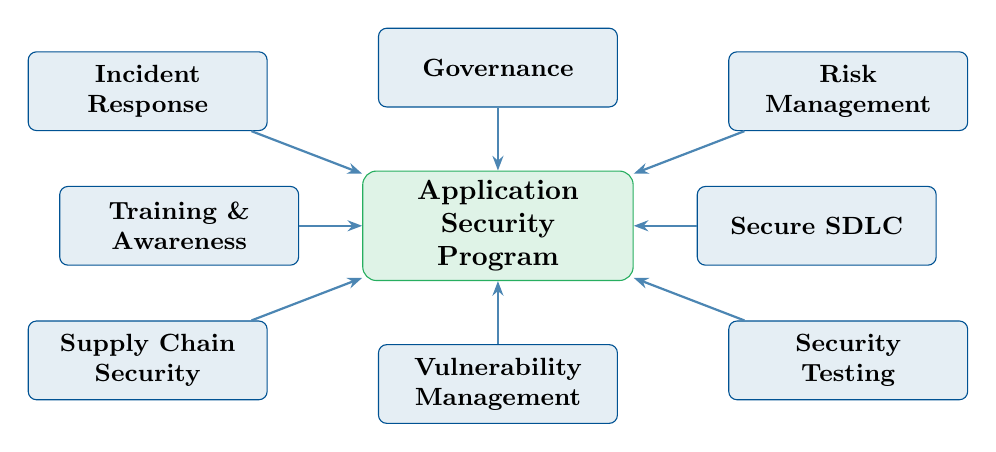
\begin{tikzpicture}[
        node distance=0.8cm,
        box/.style={rectangle, draw=primaryblue, fill=primaryblue!10, 
                    text width=2.8cm, minimum height=1cm, align=center,
                    rounded corners=3pt, font=\small\bfseries},
        centerbox/.style={rectangle, draw=accentgreen, fill=accentgreen!15, 
                    text width=3.2cm, minimum height=1.2cm, align=center,
                    rounded corners=5pt, font=\normalsize\bfseries},
        arrow/.style={-{Stealth[scale=0.8]}, thick, primaryblue!70}
    ]
        % Center node
        \node[centerbox] (center) {Application\\Security\\Program};
        
        % Surrounding nodes
        \node[box, above=of center] (gov) {Governance};
        \node[box, above right=0.5cm and 1.2cm of center] (risk) {Risk\\Management};
        \node[box, right=of center] (sdlc) {Secure SDLC};
        \node[box, below right=0.5cm and 1.2cm of center] (test) {Security\\Testing};
        \node[box, below=of center] (vuln) {Vulnerability\\Management};
        \node[box, below left=0.5cm and 1.2cm of center] (supply) {Supply Chain\\Security};
        \node[box, left=of center] (train) {Training \&\\Awareness};
        \node[box, above left=0.5cm and 1.2cm of center] (incident) {Incident\\Response};
        
        % Arrows
        \draw[arrow] (gov) -- (center);
        \draw[arrow] (risk) -- (center);
        \draw[arrow] (sdlc) -- (center);
        \draw[arrow] (test) -- (center);
        \draw[arrow] (vuln) -- (center);
        \draw[arrow] (supply) -- (center);
        \draw[arrow] (train) -- (center);
        \draw[arrow] (incident) -- (center);
    \end{tikzpicture}
    
    \vspace{1.5cm}
    
    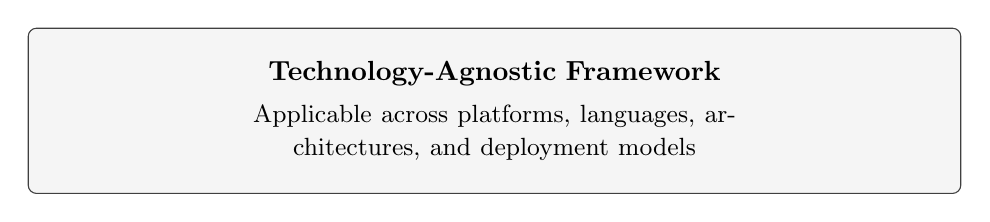
\begin{tikzpicture}
        \node[draw=darkgray, fill=lightgray, rounded corners=3pt, 
              text width=11cm, align=center, inner sep=12pt] {
            \textbf{Technology-Agnostic Framework}\\[0.3em]
            {\small Applicable across platforms, languages, architectures, and deployment models}
        };
    \end{tikzpicture}
    
    \vfill
    
    {\large\textcolor{darkgray}{Version 1.0}\par}
    \vspace{0.3cm}
    {\large\textcolor{darkgray}{\today}\par}
    
\end{titlepage}

% ============================================================================
% TABLE OF CONTENTS
% ============================================================================
\newpage
\tableofcontents
\newpage

% ============================================================================
% SECTION 1: EXECUTIVE SUMMARY
% ============================================================================
\section{Executive Summary}

This Application Security Program establishes the comprehensive framework, governance structure, processes, and controls necessary to protect the organization's software applications throughout their entire lifecycle. The program takes a technology-agnostic approach, providing principles and practices applicable across any platform, programming language, architecture, or deployment model.

\begin{keyconceptbox}[Program Mission Statement]
To systematically reduce application security risk across the enterprise by embedding security into every phase of the software development lifecycle, fostering a security-conscious culture, and establishing measurable controls that protect organizational assets, customer data, and business operations from application-layer threats.
\end{keyconceptbox}

\subsection{Program Objectives}

The Application Security Program pursues the following strategic objectives:

\begin{enumerate}[leftmargin=2em, itemsep=0.4em]
    \item \textbf{Risk Reduction:} Systematically identify, assess, and mitigate application security risks before they can be exploited, reducing the organization's overall threat exposure.
    
    \item \textbf{Secure Development:} Integrate security activities into all phases of the software development lifecycle, ensuring that security is a fundamental consideration rather than an afterthought.
    
    \item \textbf{Vulnerability Management:} Establish efficient processes for discovering, prioritizing, remediating, and verifying the closure of security vulnerabilities across the application portfolio.
    
    \item \textbf{Compliance Assurance:} Meet regulatory, contractual, and industry security requirements through documented controls, regular assessments, and audit-ready evidence.
    
    \item \textbf{Security Culture:} Build organization-wide security awareness and capability through targeted training, clear accountability, and positive reinforcement of secure practices.
    
    \item \textbf{Continuous Improvement:} Evolve program maturity through regular assessment, metrics-driven decision making, and adoption of emerging best practices.
\end{enumerate}
\clearpage

\subsection{Scope and Applicability}

This program applies to all software applications developed, acquired, deployed, or maintained by the organization, including:

\begin{itemize}[leftmargin=2em]
    \item Internally developed applications regardless of technology stack
    \item Commercial off-the-shelf (COTS) software with custom configurations
    \item Software-as-a-Service (SaaS) applications integrated into business processes
    \item Mobile applications across all platforms
    \item Application programming interfaces (APIs) both internal and external
    \item Microservices and containerized workloads
    \item Serverless functions and cloud-native applications
    \item Legacy systems and mainframe applications
    \item Third-party components and open-source libraries
    \item Infrastructure-as-code and configuration scripts
\end{itemize}

\subsection{Program Structure Overview}

\begin{figure}[H]
\centering
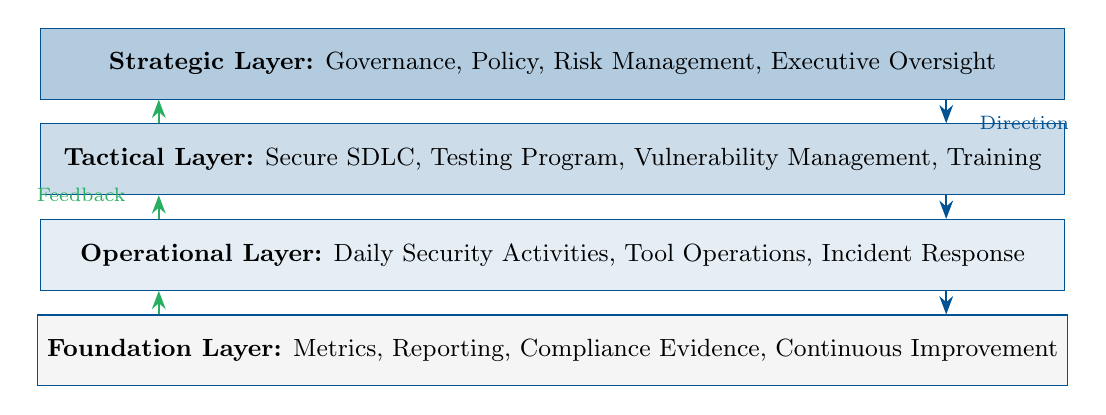
\begin{tikzpicture}[
    node distance=0.3cm,
    layer/.style={rectangle, draw=primaryblue, minimum width=13cm, minimum height=0.9cm, 
                  align=center, font=\small},
    sublayer/.style={rectangle, draw=secondaryblue!70, minimum width=4cm, minimum height=0.7cm, 
                  align=center, font=\footnotesize}
]
    % Strategic Layer
    \node[layer, fill=primaryblue!30] (strategic) {\textbf{Strategic Layer:} Governance, Policy, Risk Management, Executive Oversight};
    
    % Tactical Layer
    \node[layer, fill=primaryblue!20, below=of strategic] (tactical) {\textbf{Tactical Layer:} Secure SDLC, Testing Program, Vulnerability Management, Training};
    
    % Operational Layer
    \node[layer, fill=primaryblue!10, below=of tactical] (operational) {\textbf{Operational Layer:} Daily Security Activities, Tool Operations, Incident Response};
    
    % Foundation Layer
    \node[layer, fill=lightgray, below=of operational] (foundation) {\textbf{Foundation Layer:} Metrics, Reporting, Compliance Evidence, Continuous Improvement};
    
    % Arrows
    \draw[-{Stealth}, thick, primaryblue] ([xshift=5cm]strategic.south) -- ([xshift=5cm]tactical.north);
    \draw[-{Stealth}, thick, primaryblue] ([xshift=5cm]tactical.south) -- ([xshift=5cm]operational.north);
    \draw[-{Stealth}, thick, primaryblue] ([xshift=5cm]operational.south) -- ([xshift=5cm]foundation.north);
    
    \draw[-{Stealth}, thick, accentgreen] ([xshift=-5cm]foundation.north) -- ([xshift=-5cm]operational.south);
    \draw[-{Stealth}, thick, accentgreen] ([xshift=-5cm]operational.north) -- ([xshift=-5cm]tactical.south);
    \draw[-{Stealth}, thick, accentgreen] ([xshift=-5cm]tactical.north) -- ([xshift=-5cm]strategic.south);
    
    % Labels
    \node[right, font=\scriptsize\color{primaryblue}] at ([xshift=5.3cm]tactical.north) {Direction};
    \node[left, font=\scriptsize\color{accentgreen}] at ([xshift=-5.3cm]tactical.south) {Feedback};
\end{tikzpicture}
\caption{Application Security Program Layered Structure}
\label{fig:program-structure}
\end{figure}

% ============================================================================
% SECTION 2: GOVERNANCE FRAMEWORK
% ============================================================================
\clearpage
\section{Governance Framework}

Effective governance provides the foundation for a successful Application Security Program. This section establishes the organizational structures, roles, responsibilities, and decision-making processes that ensure security activities align with business objectives and receive appropriate oversight.

\subsection{Governance Principles}

The Application Security Program governance adheres to the following principles:

\begin{keyconceptbox}[Core Governance Principles]
\begin{enumerate}[leftmargin=1.5em, itemsep=0.3em]
    \item \textbf{Accountability:} Every security control, process, and decision has a clearly defined owner responsible for its effectiveness.
    
    \item \textbf{Transparency:} Security posture, risks, and program performance are visible to appropriate stakeholders through regular reporting.
    
    \item \textbf{Risk-Based Prioritization:} Resources and attention are allocated based on assessed risk to business objectives rather than compliance checklists alone.
    
    \item \textbf{Business Alignment:} Security requirements and activities support rather than obstruct legitimate business operations.
    
    \item \textbf{Continuous Oversight:} Regular review cycles ensure the program remains effective and adapts to changing threats and business needs.
    
    \item \textbf{Segregation of Duties:} Critical security functions maintain appropriate separation to prevent conflicts of interest and single points of failure.
\end{enumerate}
\end{keyconceptbox}

\clearpage
\subsection{Organizational Structure}

\subsubsection{Executive Sponsorship}

Executive sponsorship is essential for program success. The executive sponsor, typically a C-level officer such as the Chief Information Security Officer (CISO), Chief Technology Officer (CTO), or Chief Information Officer (CIO), provides strategic direction, secures budget allocation, removes organizational obstacles, and ensures security priorities receive appropriate attention at the executive level.

\begin{table}[H]
\centering
\renewcommand{\arraystretch}{1.3}
\begin{tabularx}{\textwidth}{>{\bfseries}p{3.5cm} X}
\toprule
\textbf{Responsibility} & \textbf{Description} \\
\midrule
Strategic Direction & Define the overall vision and strategic objectives for application security aligned with enterprise risk appetite \\
Resource Allocation & Secure and allocate budget, personnel, and tooling necessary for program execution \\
Organizational Authority & Provide the authority necessary to enforce security requirements across business units \\
Executive Communication & Report program status, risks, and achievements to the board and executive leadership \\
Conflict Resolution & Resolve disputes between security requirements and business priorities \\
Culture Leadership & Champion security as an organizational value through visible support and communication \\
\bottomrule
\end{tabularx}
\caption{Executive Sponsor Responsibilities}
\label{tab:exec-sponsor}
\end{table}

\clearpage
\subsubsection{Security Steering Committee}

The Security Steering Committee provides cross-functional oversight and governance for the Application Security Program. This body includes representatives from key stakeholder groups and meets regularly to review program performance, address strategic issues, and align security activities with business objectives.

\begin{examplebox}[Steering Committee Composition]
\begin{itemize}[leftmargin=1.5em, itemsep=0.2em]
    \item Executive Sponsor (Chair)
    \item Application Security Program Manager
    \item Engineering/Development Leadership
    \item IT Operations Leadership
    \item Enterprise Architecture Representative
    \item Legal/Compliance Representative
    \item Business Unit Representatives (rotating)
    \item Risk Management Representative
    \item Internal Audit Representative (observer)
\end{itemize}
\end{examplebox}

The Steering Committee convenes monthly for operational reviews and quarterly for strategic planning sessions. Committee responsibilities include approving program strategy and roadmap, reviewing risk acceptance decisions above defined thresholds, resolving cross-functional conflicts, evaluating program metrics and maturity assessments, and approving significant policy changes.

\subsubsection{Application Security Team Structure}

The Application Security team executes the day-to-day activities of the program. Team size and structure scale with organizational size, application portfolio complexity, and program maturity. The following model represents a mature team structure that organizations should evolve toward over time.

\begin{figure}[H]
\centering
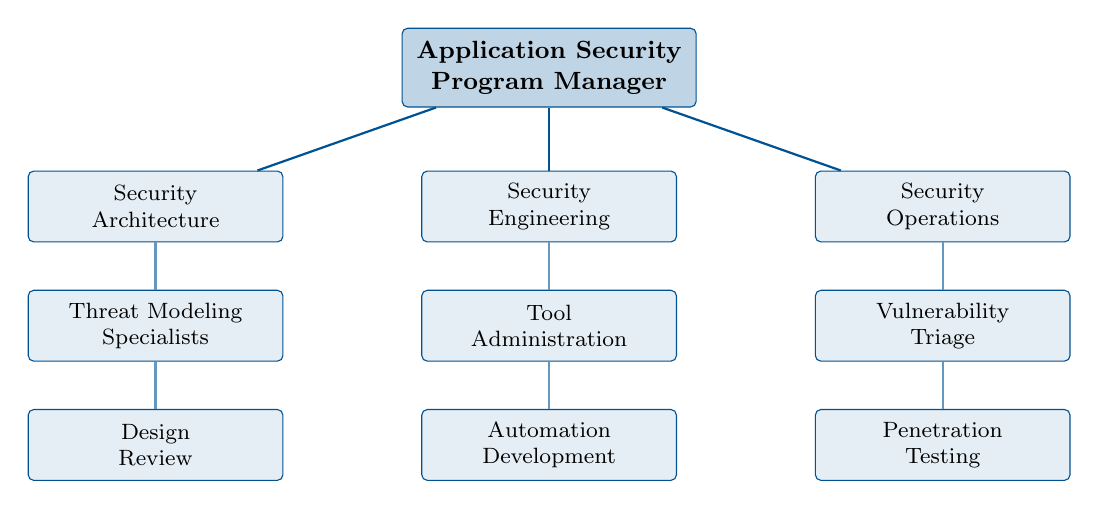
\begin{tikzpicture}[
    node distance=0.6cm and 0.3cm,
    box/.style={rectangle, draw=primaryblue, fill=primaryblue!10, 
                text width=3cm, minimum height=0.9cm, align=center,
                rounded corners=2pt, font=\footnotesize},
    leaderbox/.style={rectangle, draw=primaryblue, fill=primaryblue!25, 
                text width=3.5cm, minimum height=1cm, align=center,
                rounded corners=2pt, font=\small\bfseries}
]
    % Leader
    \node[leaderbox] (leader) {Application Security\\Program Manager};
    
    % Second level
    \node[box, below left=0.8cm and 1.5cm of leader] (arch) {Security\\Architecture};
    \node[box, below=0.8cm of leader] (eng) {Security\\Engineering};
    \node[box, below right=0.8cm and 1.5cm of leader] (ops) {Security\\Operations};
    
    % Third level
    \node[box, below=0.6cm of arch] (threat) {Threat Modeling\\Specialists};
    \node[box, below=0.6cm of eng] (tool) {Tool\\Administration};
    \node[box, below=0.6cm of ops] (triage) {Vulnerability\\Triage};
    
    \node[box, below=0.6cm of threat] (review) {Design\\Review};
    \node[box, below=0.6cm of tool] (auto) {Automation\\Development};
    \node[box, below=0.6cm of triage] (pentest) {Penetration\\Testing};
    
    % Lines
    \draw[thick, primaryblue] (leader) -- (arch);
    \draw[thick, primaryblue] (leader) -- (eng);
    \draw[thick, primaryblue] (leader) -- (ops);
    \draw[thick, primaryblue!60] (arch) -- (threat);
    \draw[thick, primaryblue!60] (eng) -- (tool);
    \draw[thick, primaryblue!60] (ops) -- (triage);
    \draw[thick, primaryblue!60] (threat) -- (review);
    \draw[thick, primaryblue!60] (tool) -- (auto);
    \draw[thick, primaryblue!60] (triage) -- (pentest);
\end{tikzpicture}
\caption{Application Security Team Organization}
\label{fig:team-structure}
\end{figure}

\clearpage
\subsection{Roles and Responsibilities}

Clear definition of roles and responsibilities ensures accountability and prevents gaps in security coverage. The following RACI matrix defines responsibility assignments for key program activities.

\begin{table}[H]
\centering
\renewcommand{\arraystretch}{1.2}
\footnotesize
\begin{tabularx}{\textwidth}{X c c c c c c}
\toprule
\textbf{Activity} & \textbf{Exec} & \textbf{AppSec} & \textbf{Dev} & \textbf{Ops} & \textbf{Legal} & \textbf{Audit} \\
\midrule
Security Policy Approval & A & R & C & C & C & I \\
Risk Assessment & A & R & C & C & I & I \\
Threat Modeling & I & A/R & R & C & --- & --- \\
Secure Code Review & I & A & R & --- & --- & --- \\
Security Testing & I & A/R & C & C & --- & I \\
Vulnerability Remediation & I & C & A/R & R & --- & I \\
Security Training & A & R & R & R & --- & --- \\
Incident Response & A & R & R & R & C & I \\
Compliance Reporting & A & R & C & C & R & R \\
Tool Selection & A & R & C & C & C & --- \\
\bottomrule
\end{tabularx}
\caption{RACI Matrix for Application Security Activities (R=Responsible, A=Accountable, C=Consulted, I=Informed)}
\label{tab:raci}
\end{table}

\subsubsection{Development Team Responsibilities}

Development teams bear primary responsibility for building secure software. This includes writing secure code, remediating identified vulnerabilities within SLA timeframes, participating in security training, incorporating security requirements into user stories and acceptance criteria, and escalating potential security concerns to the Application Security team.

\clearpage
\subsubsection{Security Champions}

Security Champions are development team members who serve as the primary security liaison between their team and the Application Security function. This distributed model extends security expertise across the organization and embeds security considerations into daily development activities.

\begin{policybox}[Security Champion Program Requirements]
\textbf{Selection Criteria:}

\begin{itemize}[leftmargin=1.5em, itemsep=0.2em]
    \item Demonstrated interest in security topics
    \item Respected technical contributor within their team
    \item Effective communicator across technical and non-technical audiences
    \item Sufficient tenure to understand team processes and codebase
\end{itemize}

\textbf{Champion Responsibilities:}

\begin{itemize}[leftmargin=1.5em, itemsep=0.2em]
    \item Participate in advanced security training (minimum 20 hours annually)
    \item Attend monthly Security Champion meetings
    \item Serve as first point of contact for security questions within the team
    \item Promote security awareness and best practices
    \item Assist with vulnerability triage and remediation prioritization
    \item Participate in threat modeling sessions for team projects
    \item Provide feedback on security tools and processes
\end{itemize}

\textbf{Program Support:}

\begin{itemize}[leftmargin=1.5em, itemsep=0.2em]
    \item Dedicated time allocation (10-20\% of capacity)
    \item Access to advanced training and certifications
    \item Recognition in performance evaluations
    \item Direct communication channel to Application Security leadership
\end{itemize}
\end{policybox}

\subsection{Policy Framework}

\subsubsection{Policy Hierarchy}

The Application Security Program operates within a hierarchical policy framework that ensures consistency while allowing appropriate flexibility at operational levels.

\begin{figure}[H]
\centering
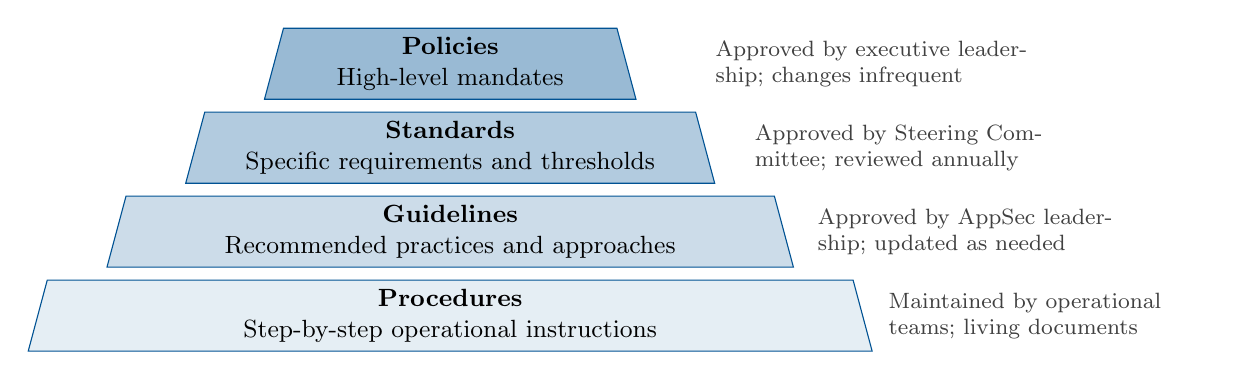
\begin{tikzpicture}[
    node distance=0.15cm,
    level/.style={trapezium, trapezium angle=75, draw=primaryblue, 
                  minimum height=0.9cm, align=center, font=\small}
]
    \node[level, fill=primaryblue!40, text width=4cm] (policy) {\textbf{Policies}\\High-level mandates};
    \node[level, fill=primaryblue!30, text width=6cm, below=of policy] (standard) {\textbf{Standards}\\Specific requirements and thresholds};
    \node[level, fill=primaryblue!20, text width=8cm, below=of standard] (guideline) {\textbf{Guidelines}\\Recommended practices and approaches};
    \node[level, fill=primaryblue!10, text width=10cm, below=of guideline] (procedure) {\textbf{Procedures}\\Step-by-step operational instructions};
    
    % Annotations
    \node[right=1cm of policy, font=\footnotesize\color{darkgray}, text width=4cm] {Approved by executive leadership; changes infrequent};
    \node[right=0.5cm of standard, font=\footnotesize\color{darkgray}, text width=4cm] {Approved by Steering Committee; reviewed annually};
    \node[right=0.3cm of guideline, font=\footnotesize\color{darkgray}, text width=4cm] {Approved by AppSec leadership; updated as needed};
    \node[right=0.2cm of procedure, font=\footnotesize\color{darkgray}, text width=4cm] {Maintained by operational teams; living documents};
\end{tikzpicture}
\caption{Policy Document Hierarchy}
\label{fig:policy-hierarchy}
\end{figure}

\clearpage
\subsubsection{Core Security Policies}

The following policies form the foundation of the Application Security Program:

\begin{longtable}{>{\bfseries}p{4cm} p{9cm}}
\toprule
\textbf{Policy} & \textbf{Scope and Purpose} \\
\midrule
\endfirsthead
\toprule
\textbf{Policy} & \textbf{Scope and Purpose} \\
\midrule
\endhead
\bottomrule
\endfoot
Secure Development Policy & Establishes requirements for integrating security into all phases of software development, including mandatory security activities, training requirements, and quality gates \\
Vulnerability Management Policy & Defines requirements for identifying, assessing, prioritizing, remediating, and reporting security vulnerabilities across the application portfolio \\
Security Testing Policy & Specifies mandatory security testing activities, frequency requirements, scope coverage, and finding management procedures \\
Third-Party Security Policy & Establishes requirements for assessing and managing security risks associated with vendor software, open-source components, and external services \\
Security Architecture Policy & Defines security design principles, approved patterns, reference architectures, and design review requirements for applications \\
Data Protection Policy & Specifies requirements for protecting sensitive data within applications, including classification, encryption, access controls, and retention \\
Authentication and Authorization Policy & Establishes requirements for identity verification, access control implementation, session management, and privilege management \\
Security Incident Response Policy & Defines procedures for detecting, analyzing, containing, and recovering from application security incidents \\
Security Exception Policy & Establishes the process for requesting, reviewing, approving, and tracking deviations from security requirements \\
Security Metrics and Reporting Policy & Defines requirements for measuring, reporting, and acting upon application security metrics \\
\end{longtable}

\clearpage
\subsubsection{Exception Management}

Security exceptions allow controlled deviation from policy requirements when business justification exists and compensating controls adequately mitigate residual risk. The exception process ensures that deviations are documented, time-limited, monitored, and approved at appropriate authority levels.

\begin{table}[H]
\centering
\renewcommand{\arraystretch}{1.3}
\begin{tabularx}{\textwidth}{>{\bfseries}p{2.5cm} p{3cm} p{3cm} X}
\toprule
\textbf{Risk Level} & \textbf{Approval Authority} & \textbf{Maximum Duration} & \textbf{Review Frequency} \\
\midrule
Critical & Executive Sponsor & 30 days & Weekly \\
High & Steering Committee & 90 days & Bi-weekly \\
Medium & AppSec Manager & 180 days & Monthly \\
Low & AppSec Team Lead & 365 days & Quarterly \\
\bottomrule
\end{tabularx}
\caption{Exception Approval Authority Matrix}
\label{tab:exception-authority}
\end{table}

Exception requests must include business justification for the deviation, risk assessment of the exception, proposed compensating controls, remediation plan with target date, and business owner acceptance of residual risk. All exceptions are tracked in a central register and reported to the Steering Committee.

% ============================================================================
% SECTION 3: RISK MANAGEMENT
% ============================================================================
\clearpage
\section{Risk Management}

Application security risk management provides the framework for identifying, assessing, prioritizing, and treating security risks across the application portfolio. This risk-based approach ensures that limited security resources focus on the highest-impact activities.

\subsection{Risk Management Framework}

\begin{figure}[H]
\centering
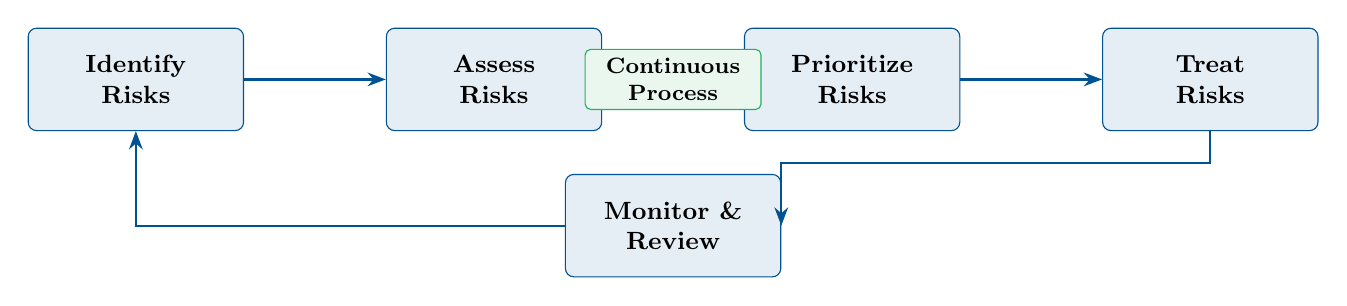
\begin{tikzpicture}[
    node distance=1.8cm,
    box/.style={rectangle, draw=primaryblue, fill=primaryblue!10, 
                text width=2.5cm, minimum height=1.3cm, align=center,
                rounded corners=3pt, font=\small\bfseries},
    arrow/.style={-{Stealth[scale=1]}, thick, primaryblue}
]
    \node[box] (identify) {Identify\\Risks};
    \node[box, right=of identify] (assess) {Assess\\Risks};
    \node[box, right=of assess] (prioritize) {Prioritize\\Risks};
    \node[box, right=of prioritize] (treat) {Treat\\Risks};
    \node[box, below=1.2cm of $(assess)!0.5!(prioritize)$] (monitor) {Monitor \&\\Review};
    
    \draw[arrow] (identify) -- (assess);
    \draw[arrow] (assess) -- (prioritize);
    \draw[arrow] (prioritize) -- (treat);
    \draw[arrow] (treat.south) -- ++(0,-0.4) -| (monitor.east);
    \draw[arrow] (monitor.west) -| ([yshift=-0.4cm]identify.south) -- (identify.south);
    
    % Central element
    \node[draw=accentgreen, fill=accentgreen!10, rounded corners=2pt, 
          text width=2cm, align=center, font=\footnotesize\bfseries] 
          at ($(assess)!0.5!(prioritize)$) {Continuous\\Process};
\end{tikzpicture}
\caption{Risk Management Lifecycle}
\label{fig:risk-lifecycle}
\end{figure}

\subsection{Risk Identification}

Risk identification systematically discovers potential threats to application security. Sources for risk identification include:

\begin{itemize}[leftmargin=2em]
    \item Threat intelligence feeds and industry reports
    \item Vulnerability scan and penetration test results
    \item Security incident post-mortems
    \item Architecture and design reviews
    \item Threat modeling exercises
    \item Audit findings and compliance assessments
    \item Third-party security assessments
    \item Bug bounty program submissions
    \item Developer and operations team input
    \item Changes in regulatory or contractual requirements
\end{itemize}

\clearpage
\subsection{Risk Assessment Methodology}

Risk assessment evaluates identified risks based on likelihood of occurrence and potential impact to the organization. This program uses a semi-quantitative approach that balances rigor with practicality.

\subsubsection{Likelihood Assessment}

Likelihood reflects the probability that a vulnerability will be exploited or a threat will materialize, considering threat actor capability and motivation, exposure and accessibility of the vulnerable component, existing controls and their effectiveness, and historical incident data.

\begin{table}[H]
\centering
\renewcommand{\arraystretch}{1.3}
\begin{tabularx}{\textwidth}{>{\bfseries\centering\arraybackslash}p{2cm} >{\centering\arraybackslash}p{1.5cm} X}
\toprule
\textbf{Level} & \textbf{Score} & \textbf{Description} \\
\midrule
Very High & 5 & Exploitation expected; active exploitation observed in the wild; trivial to exploit \\
High & 4 & Exploitation likely; exploit code available; minimal skill required \\
Medium & 3 & Exploitation possible; requires moderate skill or specific conditions \\
Low & 2 & Exploitation unlikely; requires significant skill, access, or rare conditions \\
Very Low & 1 & Exploitation improbable; theoretical only or requires extraordinary circumstances \\
\bottomrule
\end{tabularx}
\caption{Likelihood Rating Scale}
\label{tab:likelihood}
\end{table}

\subsubsection{Impact Assessment}

Impact assessment considers multiple dimensions of potential harm:

\begin{table}[H]
\centering
\renewcommand{\arraystretch}{1.3}
\begin{tabularx}{\textwidth}{>{\bfseries\raggedright\arraybackslash}p{3.4cm} X}
\toprule
\textbf{Impact Category} & \textbf{Considerations} \\
\midrule
Financial & Direct financial loss, regulatory fines, remediation costs, legal liability \\
Operational & Business process disruption, system availability, recovery time \\
Reputational & Customer trust, brand damage, media exposure, market position \\
Legal/Regulatory & Compliance violations, contractual breaches, litigation exposure \\
Safety & Physical safety of individuals, environmental impact \\
Data & Confidentiality breach scope, data sensitivity, affected individuals \\
\bottomrule
\end{tabularx}
\caption{Impact Assessment Categories}
\label{tab:impact-categories}
\end{table}

\begin{table}[H]
\centering
\renewcommand{\arraystretch}{1.3}
\begin{tabularx}{\textwidth}{>{\bfseries\centering\arraybackslash}p{2cm} >{\centering\arraybackslash}p{1.5cm} X}
\toprule
\textbf{Level} & \textbf{Score} & \textbf{Description} \\
\midrule
Critical & 5 & Existential threat to organization; massive breach; regulatory shutdown \\
High & 4 & Major financial loss; significant breach; substantial regulatory action \\
Medium & 3 & Moderate financial impact; limited breach; regulatory inquiry \\
Low & 2 & Minor financial impact; minimal data exposure; internal concern \\
Minimal & 1 & Negligible impact; no data exposure; no regulatory implications \\
\bottomrule
\end{tabularx}
\caption{Impact Rating Scale}
\label{tab:impact}
\end{table}

\subsubsection{Risk Scoring}

Risk score is calculated as the product of likelihood and impact scores, producing a value between 1 and 25:

\begin{figure}[H]
\centering
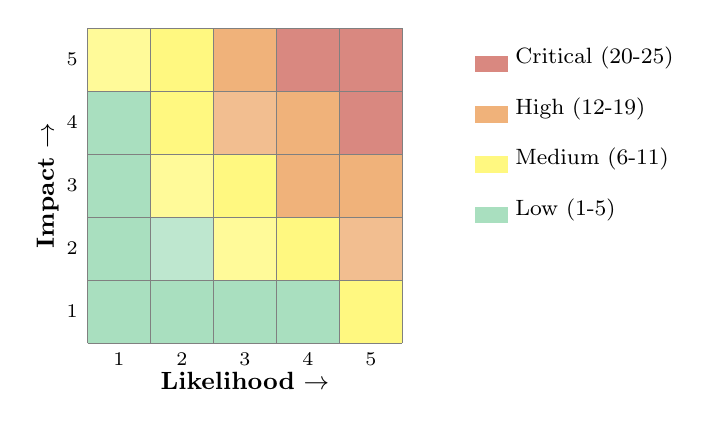
\begin{tikzpicture}[scale=0.8]
    % Grid
    \foreach \x in {0,1,2,3,4,5} {
        \draw[gray!50] (\x,0) -- (\x,5);
        \draw[gray!50] (0,\x) -- (5,\x);
    }
    
    % Color cells based on risk
    % Critical (20-25): Red
    \fill[alertred!60] (4,3) rectangle (5,5);
    \fill[alertred!60] (3,4) rectangle (4,5);
    
    % High (12-19): Orange
    \fill[warningorange!60] (2,4) rectangle (3,5);
    \fill[warningorange!60] (3,3) rectangle (4,4);
    \fill[warningorange!60] (4,2) rectangle (5,3);
    \fill[warningorange!60] (3,2) rectangle (4,3);
    \fill[warningorange!50] (4,1) rectangle (5,2);
    \fill[warningorange!50] (2,3) rectangle (3,4);
    
    % Medium (6-11): Yellow
    \fill[yellow!50] (1,4) rectangle (2,5);
    \fill[yellow!50] (2,2) rectangle (3,3);
    \fill[yellow!50] (1,3) rectangle (2,4);
    \fill[yellow!50] (3,1) rectangle (4,2);
    \fill[yellow!50] (4,0) rectangle (5,1);
    \fill[yellow!40] (0,4) rectangle (1,5);
    \fill[yellow!40] (1,2) rectangle (2,3);
    \fill[yellow!40] (2,1) rectangle (3,2);
    
    % Low (1-5): Green
    \fill[accentgreen!40] (0,0) rectangle (1,4);
    \fill[accentgreen!40] (1,0) rectangle (2,2);
    \fill[accentgreen!40] (2,0) rectangle (3,1);
    \fill[accentgreen!40] (3,0) rectangle (4,1);
    \fill[accentgreen!30] (1,1) rectangle (2,2);
    
    % Grid lines on top
    \foreach \x in {0,1,2,3,4,5} {
        \draw[gray] (\x,0) -- (\x,5);
        \draw[gray] (0,\x) -- (5,\x);
    }
    
    % Labels
    \node[below, font=\small] at (2.5,-0.3) {\textbf{Likelihood} $\rightarrow$};
    \node[rotate=90, above, font=\small] at (-0.3,2.5) {\textbf{Impact} $\rightarrow$};
    
    % Axis labels
    \foreach \x/\label in {0.5/1, 1.5/2, 2.5/3, 3.5/4, 4.5/5} {
        \node[below, font=\scriptsize] at (\x,0) {\label};
        \node[left, font=\scriptsize] at (0,\x) {\label};
    }
    
    % Legend
    \node[right, font=\footnotesize] at (6,4.5) {\colorbox{alertred!60}{\ \ } Critical (20-25)};
    \node[right, font=\footnotesize] at (6,3.7) {\colorbox{warningorange!60}{\ \ } High (12-19)};
    \node[right, font=\footnotesize] at (6,2.9) {\colorbox{yellow!50}{\ \ } Medium (6-11)};
    \node[right, font=\footnotesize] at (6,2.1) {\colorbox{accentgreen!40}{\ \ } Low (1-5)};
\end{tikzpicture}
\caption{Risk Scoring Matrix}
\label{fig:risk-matrix}
\end{figure}

\clearpage
\subsection{Risk Appetite and Tolerance}

Risk appetite defines the aggregate level of risk the organization is willing to accept in pursuit of its objectives. Risk tolerance defines acceptable variation around specific risk categories or activities.

\begin{alertbox}[Risk Appetite Statement]
The organization maintains a \textbf{conservative risk appetite} for application security, recognizing that application-layer vulnerabilities represent a primary attack vector and that security incidents can cause significant financial, reputational, and regulatory harm. The organization accepts that some residual risk is unavoidable but commits to maintaining risk within defined tolerance levels through systematic identification, assessment, and mitigation of application security risks.
\end{alertbox}

\begin{table}[H]
\centering
\renewcommand{\arraystretch}{1.3}
\begin{tabularx}{\textwidth}{>{\bfseries}p{2.5cm} >{\centering\arraybackslash}p{2cm} X}
\toprule
\textbf{Risk Category} & \textbf{Tolerance} & \textbf{Rationale} \\
\midrule
Critical Vulnerabilities & Zero & No critical vulnerabilities accepted in production systems \\
High Vulnerabilities & Very Low & Limited tolerance with strict SLA and executive visibility \\
Data Breach Risk & Very Low & Strict controls required for all sensitive data processing \\
Compliance Risk & Low & Regulatory violations carry significant penalties \\
Third-Party Risk & Moderate & Accept managed risk for business-critical vendors \\
Emerging Technology Risk & Moderate & Accept higher uncertainty for innovation initiatives \\
\bottomrule
\end{tabularx}
\caption{Risk Tolerance by Category}
\label{tab:risk-tolerance}
\end{table}

\clearpage
\subsection{Risk Treatment}

Risk treatment selects and implements controls to modify risk. Four treatment options exist:

\begin{keyconceptbox}[Risk Treatment Options]
\textbf{Avoid:} Eliminate the risk by discontinuing the activity or removing the vulnerable component. Appropriate when risk exceeds appetite and no acceptable mitigation exists.

\textbf{Mitigate:} Implement controls to reduce likelihood or impact. The primary treatment option for most application security risks.

\textbf{Transfer:} Share risk with third parties through insurance, contracts, or outsourcing. Does not eliminate risk but redistributes financial consequences.

\textbf{Accept:} Acknowledge and monitor risk without additional controls. Requires documented acceptance by appropriate authority based on risk level.
\end{keyconceptbox}

\subsection{Application Risk Classification}

Applications are classified based on their risk profile to ensure appropriate security treatment. Classification considers data sensitivity, business criticality, exposure, and regulatory requirements.

\begin{table}[H]
\centering
\renewcommand{\arraystretch}{1.3}
\begin{tabularx}{\textwidth}{>{\bfseries\centering\arraybackslash}p{2cm} X p{4.5cm}}
\toprule
\textbf{Tier} & \textbf{Criteria} & \textbf{Security Requirements} \\
\midrule
Tier 1 (Critical) & Processes highly sensitive data; revenue-critical; customer-facing; regulatory scope & Full security testing suite; annual penetration test; threat modeling; security architecture review; continuous monitoring \\
Tier 2 (High) & Processes sensitive data; supports critical business functions; internal enterprise applications & SAST/DAST; periodic penetration testing; security design review; vulnerability scanning \\
Tier 3 (Medium) & Processes internal data; supports departmental functions; limited exposure & Automated security scanning; standard secure development practices; risk-based testing \\
Tier 4 (Low) & Minimal data processing; limited business impact; no external exposure & Basic security hygiene; standard development practices; periodic review \\
\bottomrule
\end{tabularx}
\caption{Application Risk Classification Tiers}
\label{tab:app-tiers}
\end{table}

% ============================================================================
% SECTION 4: SECURE SOFTWARE DEVELOPMENT LIFECYCLE
% ============================================================================
\clearpage
\section{Secure Software Development Lifecycle}

The Secure Software Development Lifecycle (SSDLC) integrates security activities into every phase of software development, ensuring that security is considered from initial concept through retirement. This section defines mandatory security activities, quality gates, and deliverables for each lifecycle phase.

\subsection{SSDLC Overview}

\begin{figure}[H]
\centering
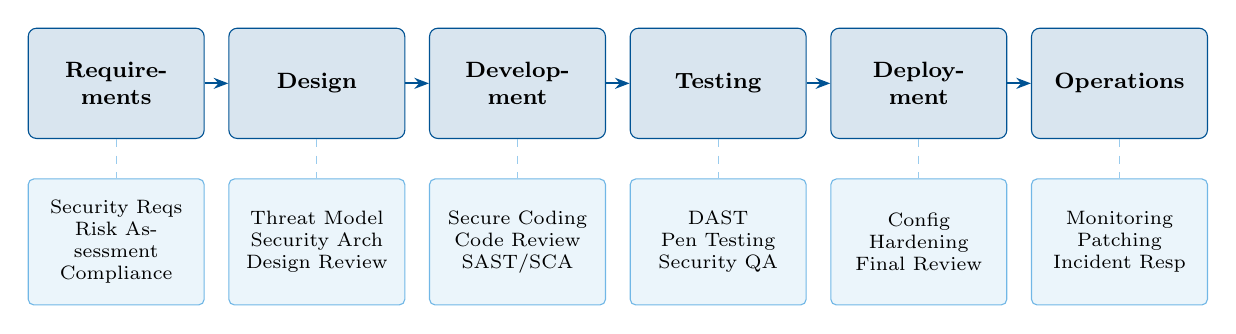
\begin{tikzpicture}[
    node distance=0.3cm,
    phase/.style={rectangle, draw=primaryblue, fill=primaryblue!15, 
                  text width=2cm, minimum height=1.4cm, align=center,
                  rounded corners=3pt, font=\footnotesize\bfseries},
    activity/.style={rectangle, draw=secondaryblue!70, fill=secondaryblue!10, 
                  text width=2cm, minimum height=1.6cm, align=center,
                  rounded corners=2pt, font=\scriptsize},
    arrow/.style={-{Stealth[scale=0.8]}, thick, primaryblue}
]
    % Phases
    \node[phase] (req) {Require-\\ments};
    \node[phase, right=of req] (design) {Design};
    \node[phase, right=of design] (dev) {Develop-\\ment};
    \node[phase, right=of dev] (test) {Testing};
    \node[phase, right=of test] (deploy) {Deploy-\\ment};
    \node[phase, right=of deploy] (ops) {Operations};
    
    % Arrows
    \draw[arrow] (req) -- (design);
    \draw[arrow] (design) -- (dev);
    \draw[arrow] (dev) -- (test);
    \draw[arrow] (test) -- (deploy);
    \draw[arrow] (deploy) -- (ops);
    
    % Security activities
    \node[activity, below=0.5cm of req] (req-act) {Security Reqs\\Risk Assessment\\Compliance};
    \node[activity, below=0.5cm of design] (design-act) {Threat Model\\Security Arch\\Design Review};
    \node[activity, below=0.5cm of dev] (dev-act) {Secure Coding\\Code Review\\SAST/SCA};
    \node[activity, below=0.5cm of test] (test-act) {DAST\\Pen Testing\\Security QA};
    \node[activity, below=0.5cm of deploy] (deploy-act) {Config\\Hardening\\Final Review};
    \node[activity, below=0.5cm of ops] (ops-act) {Monitoring\\Patching\\Incident Resp};
    
    % Connecting lines
    \draw[dashed, secondaryblue!50] (req) -- (req-act);
    \draw[dashed, secondaryblue!50] (design) -- (design-act);
    \draw[dashed, secondaryblue!50] (dev) -- (dev-act);
    \draw[dashed, secondaryblue!50] (test) -- (test-act);
    \draw[dashed, secondaryblue!50] (deploy) -- (deploy-act);
    \draw[dashed, secondaryblue!50] (ops) -- (ops-act);
\end{tikzpicture}
\caption{Secure Software Development Lifecycle with Security Activities}
\label{fig:ssdlc}
\end{figure}

\subsection{Requirements Phase}

The requirements phase establishes security requirements alongside functional requirements, ensuring security considerations are addressed from project inception.

\subsubsection{Security Requirements Identification}

Security requirements derive from multiple sources:

\begin{itemize}[leftmargin=2em]
    \item \textbf{Regulatory Requirements:} Mandates from applicable regulations such as data protection laws, industry-specific requirements, and international standards
    \item \textbf{Contractual Obligations:} Security commitments in customer contracts, service level agreements, and partnership arrangements
    \item \textbf{Organizational Policies:} Internal security policies, standards, and guidelines applicable to the application type and data classification
    \item \textbf{Threat Landscape:} Known threats and attack patterns relevant to the application's technology and business domain
    \item \textbf{Data Classification:} Requirements driven by the sensitivity of data the application will process, store, or transmit
    \item \textbf{Business Risk Assessment:} Security controls necessary to protect business value and maintain stakeholder confidence
\end{itemize}

\subsubsection{Security Requirements Categories}

\begin{table}[H]
\centering
\renewcommand{\arraystretch}{1.3}
\begin{tabularx}{\textwidth}{>{\bfseries\raggedright\arraybackslash}p{3.5cm} X}
\toprule
\textbf{Category} & \textbf{Example Requirements} \\
\midrule
Authentication & Multi-factor authentication for privileged access; session timeout after inactivity; password complexity requirements \\
Authorization & Role-based access control; principle of least privilege; segregation of duties for sensitive functions \\
Input Validation & Server-side validation of all input; parameterized queries; output encoding \\
Cryptography & Encryption of sensitive data at rest and in transit; approved algorithms and key lengths; key management procedures \\
Logging \& Monitoring & Security event logging; audit trail integrity; alerting for suspicious activities \\
Error Handling & Secure error messages; exception handling without information leakage \\
Data Protection & Data minimization; retention limits; secure deletion; anonymization requirements \\
Session Management & Secure session token generation; session binding; timeout enforcement \\
Communication Sec. & TLS for all external communications; certificate validation; secure protocols only \\
Configuration & Secure defaults; hardening requirements; change management controls \\
\bottomrule
\end{tabularx}
\caption{Security Requirements Categories}
\label{tab:sec-req-categories}
\end{table}

\subsubsection{Requirements Phase Deliverables}

\begin{examplebox}[Requirements Phase Security Deliverables]
\begin{itemize}[leftmargin=1.5em, itemsep=0.2em]
    \item Security requirements specification document
    \item Data classification determination
    \item Application risk tier classification
    \item Preliminary compliance requirements mapping
    \item Initial risk assessment
    \item Security acceptance criteria for user stories
    \item Abuse case documentation (misuse cases)
\end{itemize}
\end{examplebox}

\clearpage
\subsection{Design Phase}

The design phase translates security requirements into secure architecture and design specifications. Security decisions made during design have the greatest leverage for preventing vulnerabilities cost-effectively.

\subsubsection{Security Architecture Principles}

All application designs should adhere to established security architecture principles:

\begin{keyconceptbox}[Security Architecture Principles]
\begin{enumerate}[leftmargin=1.5em, itemsep=0.3em]
    \item \textbf{Defense in Depth:} Implement multiple layers of security controls so that failure of any single control does not compromise security
    
    \item \textbf{Least Privilege:} Grant minimum permissions necessary for each component, user, and process to perform its intended function
    
    \item \textbf{Secure Defaults:} Configure systems to be secure out of the box; require explicit action to reduce security
    
    \item \textbf{Fail Secure:} Design systems to fail in a secure state; deny access when controls fail
    
    \item \textbf{Separation of Duties:} Divide critical functions among multiple components or individuals to prevent single points of compromise
    
    \item \textbf{Economy of Mechanism:} Keep security designs as simple as possible; complexity increases attack surface and error likelihood
    
    \item \textbf{Complete Mediation:} Verify authorization for every access attempt; never rely on cached permissions
    
    \item \textbf{Open Design:} Security should not depend on secrecy of design; assume adversaries know the system architecture
    
    \item \textbf{Psychological Acceptability:} Security mechanisms should not impede legitimate use or users will circumvent them
    
    \item \textbf{Weakest Link:} Security is only as strong as the weakest component; identify and strengthen weak points
\end{enumerate}
\end{keyconceptbox}

\clearpage
\subsubsection{Threat Modeling}

Threat modeling systematically identifies potential threats to an application and determines appropriate countermeasures. All Tier 1 and Tier 2 applications require formal threat modeling during design.

\begin{table}[H]
\centering
\renewcommand{\arraystretch}{1.3}
\begin{tabularx}{\textwidth}{>{\bfseries\raggedright\arraybackslash}p{3.5cm} X}
\toprule
\textbf{Activity} & \textbf{Description} \\
\midrule
Scope Definition & Define the boundaries of analysis; identify assets, entry points, and trust boundaries \\
Decomposition & Create architectural diagrams showing components, data flows, and trust levels \\
Threat Identification & Systematically identify threats using structured approaches such as STRIDE or attack trees \\
Vulnerability Analysis & Identify potential vulnerabilities that could enable identified threats \\
Countermeasure Design & Specify controls to prevent, detect, or respond to identified threats \\
Risk Assessment & Evaluate residual risk after countermeasures; prioritize based on risk score \\
Documentation & Record threat model artifacts for future reference and updates \\
\bottomrule
\end{tabularx}
\caption{Threat Modeling Process Steps}
\label{tab:threat-model-steps}
\end{table}

\begin{notebox}[Threat Modeling Triggers]
Beyond initial design, threat modeling should be revisited when:

\begin{itemize}[leftmargin=1.5em, itemsep=0.2em]
    \item Significant architectural changes occur
    \item New data types or sensitivity levels are introduced
    \item External interfaces or integrations are added
    \item Trust boundaries are modified
    \item New threat intelligence indicates emerging attack patterns
    \item Major security incidents affect similar applications
\end{itemize}
\end{notebox}

\clearpage
\subsubsection{Security Design Review}

Security design reviews evaluate proposed architectures against security requirements and best practices. Review depth scales with application risk tier.

\begin{table}[H]
\centering
\renewcommand{\arraystretch}{1.3}
\begin{tabularx}{\textwidth}{>{\bfseries}p{2cm} p{4cm} X}
\toprule
\textbf{App Tier} & \textbf{Review Type} & \textbf{Requirements} \\
\midrule
Tier 1 & Full security architecture review & Formal review by security architecture team; documented approval required before development \\
Tier 2 & Standard design review & Review by Application Security team member; threat model validation \\
Tier 3 & Lightweight review & Security Champion review with AppSec consultation as needed \\
Tier 4 & Self-assessment & Development team completes security design checklist \\
\bottomrule
\end{tabularx}
\caption{Design Review Requirements by Application Tier}
\label{tab:design-review}
\end{table}

\subsubsection{Design Phase Deliverables}

\begin{examplebox}[Design Phase Security Deliverables]
\begin{itemize}[leftmargin=1.5em, itemsep=0.2em]
    \item Security architecture document
    \item Threat model with identified threats and countermeasures
    \item Data flow diagrams with trust boundaries
    \item Security design review approval
    \item Updated risk assessment
    \item Authentication and authorization design
    \item Cryptographic design specification
    \item Security control specifications
\end{itemize}
\end{examplebox}

\clearpage
\subsection{Development Phase}

The development phase implements the secure design through secure coding practices, code review, and automated security analysis. This phase has the highest volume of security activities but benefits from automation to maintain development velocity.

\subsubsection{Secure Coding Practices}

Developers must follow secure coding standards that address common vulnerability categories:

\begin{longtable}{>{\bfseries}p{3cm} p{10cm}}
\toprule
\textbf{Vulnerability Category} & \textbf{Secure Coding Requirements} \\
\midrule
\endfirsthead
\toprule
\textbf{Vulnerability Category} & \textbf{Secure Coding Requirements} \\
\midrule
\endhead
\bottomrule
\endfoot
Injection & Use parameterized queries for all database access; validate and sanitize all input; use safe APIs that avoid shell interpretation; implement appropriate output encoding \\
Broken Authentication & Use proven authentication frameworks; implement proper password storage with modern hashing algorithms; enforce session management controls; protect credentials in transit and storage \\
Sensitive Data Exposure & Classify data appropriately; encrypt sensitive data at rest and in transit; minimize data collection and retention; implement proper key management \\
XML External Entities & Disable external entity processing; use less complex data formats where possible; validate and sanitize XML input \\
Broken Access Control & Implement server-side authorization checks; deny by default; validate permissions on every request; log access control failures \\
Security Misconfiguration & Follow hardening guides; remove unnecessary features; keep dependencies updated; use secure defaults \\
Cross-Site Scripting & Encode output appropriately for context; use security-focused templating engines; implement Content Security Policy; validate and sanitize input \\
Insecure Deserialization & Avoid deserializing untrusted data; implement integrity checks; use simple data formats; isolate deserialization code \\
Vulnerable Components & Maintain software bill of materials; monitor for vulnerabilities; update components promptly; evaluate component security before adoption \\
Insufficient Logging & Log security-relevant events; protect log integrity; include sufficient context; enable monitoring and alerting \\
\end{longtable}

\clearpage
\subsubsection{Code Review}

Code review provides human verification of security practices that automated tools may miss. Security-focused code review examines authentication and authorization implementation, cryptographic usage, input validation and output encoding, error handling and logging, business logic security, and compliance with secure coding standards.

All code changes to Tier 1 and Tier 2 applications require security-aware code review before merge. Code reviewers must complete secure code review training and use security-focused review checklists.

\subsubsection{Static Application Security Testing (SAST)}

Static analysis examines source code or compiled binaries to identify potential security vulnerabilities without executing the application. SAST integration requirements:

\begin{policybox}[SAST Integration Requirements]
\begin{itemize}[leftmargin=1.5em, itemsep=0.2em]
    \item SAST scanning integrated into CI/CD pipeline for all repositories
    \item Scans execute on every code commit or pull request
    \item Critical and high severity findings block build progression for Tier 1 and Tier 2 applications
    \item Findings triaged within defined SLA based on severity
    \item False positives documented and suppressed with justification
    \item Custom rules implemented for organization-specific patterns
    \item Regular tuning to minimize false positives while maintaining detection
\end{itemize}
\end{policybox}

\clearpage
\subsubsection{Software Composition Analysis (SCA)}

SCA identifies security vulnerabilities and license compliance issues in third-party and open-source components. Given that modern applications typically consist of 70-90\% third-party code, SCA is essential for comprehensive coverage.

\begin{table}[H]
\centering
\renewcommand{\arraystretch}{1.3}
\begin{tabularx}{\textwidth}{>{\bfseries}p{3cm} X}
\toprule
\textbf{SCA Capability} & \textbf{Requirements} \\
\midrule
Component Inventory & Automated discovery and inventory of all direct and transitive dependencies \\
Vulnerability Detection & Real-time matching against vulnerability databases with continuous monitoring \\
License Compliance & Identification of license types and flagging of incompatible or restricted licenses \\
Version Currency & Identification of outdated components with available updates \\
Risk Scoring & Risk assessment considering vulnerability severity, exploitability, and component usage \\
Remediation Guidance & Recommended versions, upgrade paths, and workarounds \\
SBOM Generation & Automated generation of software bill of materials in standard formats \\
\bottomrule
\end{tabularx}
\caption{SCA Capability Requirements}
\label{tab:sca-capabilities}
\end{table}

\subsubsection{Secrets Management}

Credentials, API keys, certificates, and other secrets must never be committed to source code repositories. Development practices must include:

\begin{itemize}[leftmargin=2em]
    \item Pre-commit hooks to detect potential secrets in code
    \item Secrets scanning integrated into CI/CD pipelines
    \item Centralized secrets management for all environments
    \item Environment-specific secrets injection at runtime
    \item Immediate rotation of any secrets detected in repositories
    \item Regular secrets inventory and rotation
\end{itemize}

\subsubsection{Development Phase Deliverables}

\begin{examplebox}[Development Phase Security Deliverables]
\begin{itemize}[leftmargin=1.5em, itemsep=0.2em]
    \item SAST scan reports with resolved findings
    \item SCA scan reports with resolved findings
    \item Code review records with security sign-off
    \item Updated software bill of materials
    \item Secrets scan verification
    \item Unit tests for security controls
    \item Security-relevant code documentation
\end{itemize}
\end{examplebox}

\clearpage
\subsection{Testing Phase}

The testing phase validates that security controls function as designed through dynamic testing, penetration testing, and security-focused quality assurance.

\subsubsection{Dynamic Application Security Testing (DAST)}

DAST tests running applications by simulating attacks to identify runtime vulnerabilities. Unlike SAST, DAST finds vulnerabilities in deployed configurations and runtime behavior.

\begin{table}[H]
\centering
\renewcommand{\arraystretch}{1.3}
\begin{tabularx}{\textwidth}{>{\bfseries}p{3cm} X}
\toprule
\textbf{DAST Element} & \textbf{Requirements} \\
\midrule
Scan Frequency & Automated scans in CI/CD for every deployment to test environments; weekly scans of production applications \\
Coverage & Full crawl and scan of all application endpoints; authenticated scanning with appropriate credentials \\
Test Categories & OWASP Top 10 coverage; injection testing; authentication bypass; authorization testing; session management \\
Finding Handling & Automatic ticket creation for verified findings; integration with vulnerability management system \\
False Positive Management & Triage and documentation of false positives; tuning to improve accuracy \\
Environment Considerations & Scanning against representative test environments; production scanning during low-traffic periods \\
\bottomrule
\end{tabularx}
\caption{DAST Program Requirements}
\label{tab:dast-requirements}
\end{table}

\subsubsection{Interactive Application Security Testing (IAST)}

IAST combines elements of SAST and DAST by using agents deployed within the running application to monitor code execution during testing. IAST provides:

\begin{itemize}[leftmargin=2em]
    \item Real-time vulnerability detection during functional testing
    \item Precise identification of vulnerable code locations
    \item Lower false positive rates than standalone SAST or DAST
    \item Coverage of data flow through the entire application stack
    \item Integration with existing functional test suites
\end{itemize}

IAST deployment is recommended for Tier 1 and Tier 2 applications where the additional accuracy and precision justify the integration effort.

\clearpage
\subsubsection{Penetration Testing}

Penetration testing simulates real-world attacks by skilled testers to identify vulnerabilities that automated tools may miss. The penetration testing program includes:

\begin{table}[H]
\centering
\renewcommand{\arraystretch}{1.3}
\begin{tabularx}{\textwidth}{>{\bfseries}p{2cm} p{2.5cm} p{3cm} X}
\toprule
\textbf{App Tier} & \textbf{Test Type} & \textbf{Frequency} & \textbf{Scope} \\
\midrule
Tier 1 & Full penetration test & Annual minimum; after major changes & Complete application including infrastructure; red team exercises \\
Tier 2 & Application penetration test & Annual minimum & Application layer focus; API testing \\
Tier 3 & Targeted assessment & Every 2 years & Risk-based scope; specific functionality \\
Tier 4 & On request & As warranted & Based on significant changes or concerns \\
\bottomrule
\end{tabularx}
\caption{Penetration Testing Requirements by Application Tier}
\label{tab:pentest-requirements}
\end{table}

\subsubsection{Security Test Case Development}

Security test cases should be developed alongside functional test cases to verify security requirements and control implementations:

\begin{itemize}[leftmargin=2em]
    \item Authentication test cases verifying proper credential handling and session management
    \item Authorization test cases confirming access control enforcement
    \item Input validation test cases with malicious input patterns
    \item Boundary condition tests for security-relevant functions
    \item Negative test cases verifying proper denial of unauthorized actions
    \item Regression tests for previously identified vulnerabilities
\end{itemize}

\subsubsection{Testing Phase Deliverables}

\begin{examplebox}[Testing Phase Security Deliverables]
\begin{itemize}[leftmargin=1.5em, itemsep=0.2em]
    \item DAST scan reports with resolved findings
    \item IAST analysis results (where applicable)
    \item Penetration test report with remediation status
    \item Security test case execution results
    \item Security regression test results
    \item Updated risk assessment with test findings
    \item Security sign-off for release
\end{itemize}
\end{examplebox}

\subsection{Deployment Phase}

The deployment phase ensures secure configuration and hardening before applications enter production.

\subsubsection{Security Configuration Management}

All applications must be deployed with secure configurations verified against hardening baselines:

\begin{itemize}[leftmargin=2em]
    \item Security configuration baselines documented for each technology stack
    \item Automated configuration scanning to detect deviations
    \item Change management controls for security-relevant configurations
    \item Separation of configuration from code
    \item Environment-specific security controls appropriately configured
    \item Removal of default credentials, sample data, and development artifacts
\end{itemize}

\subsubsection{Deployment Security Checklist}

\begin{policybox}[Pre-Production Security Checklist]
\textbf{Code Security:}

\begin{itemize}[leftmargin=1.5em, itemsep=0.1em]
    \item All critical and high SAST findings remediated or accepted
    \item All critical and high SCA findings remediated or accepted
    \item Secrets scanning verified clean
    \item Security code review completed
\end{itemize}

\textbf{Testing Security:}

\begin{itemize}[leftmargin=1.5em, itemsep=0.1em]
    \item DAST scan completed with findings addressed
    \item Penetration test completed (per tier requirements)
    \item Security test cases passed
    \item No known critical or high vulnerabilities
\end{itemize}

\textbf{Configuration Security:}

\begin{itemize}[leftmargin=1.5em, itemsep=0.1em]
    \item Hardening baseline applied and verified
    \item TLS configuration validated
    \item Security headers configured
    \item Logging and monitoring enabled
    \item Access controls configured
\end{itemize}

\textbf{Documentation:}

\begin{itemize}[leftmargin=1.5em, itemsep=0.1em]
    \item Security architecture documentation current
    \item Runbook includes security procedures
    \item Incident response procedures documented
    \item Risk acceptance documented for residual risks
\end{itemize}
\end{policybox}

\clearpage
\subsubsection{Security Gate Approval}

Deployment to production requires security gate approval based on application tier:

\begin{table}[H]
\centering
\renewcommand{\arraystretch}{1.3}
\begin{tabularx}{\textwidth}{>{\bfseries}p{2cm} p{4cm} X}
\toprule
\textbf{App Tier} & \textbf{Approval Authority} & \textbf{Requirements} \\
\midrule
Tier 1 & Application Security Manager & All checklist items verified; penetration test current; formal sign-off \\
Tier 2 & Application Security Team Lead & Security checklist completed; SAST/DAST/SCA clear \\
Tier 3 & Security Champion & Automated scans passing; checklist self-assessment \\
Tier 4 & Development Team Lead & Automated security gates passing \\
\bottomrule
\end{tabularx}
\caption{Security Gate Approval Requirements}
\label{tab:security-gate}
\end{table}

\clearpage
\subsection{Operations and Maintenance Phase}

Security activities continue throughout the operational life of applications, addressing emerging threats, newly discovered vulnerabilities, and ongoing compliance requirements.

\subsubsection{Continuous Security Monitoring}

Production applications require ongoing security monitoring:

\begin{itemize}[leftmargin=2em]
    \item Runtime application self-protection (RASP) for Tier 1 applications
    \item Web application firewall (WAF) protection for internet-facing applications
    \item Security event logging with SIEM integration
    \item Anomaly detection for application behavior
    \item Regular vulnerability scanning of production systems
    \item Certificate expiration monitoring
    \item Dependency vulnerability monitoring
\end{itemize}

\subsubsection{Patch and Update Management}

Security patches and updates must be applied within defined timeframes:

\begin{table}[H]
\centering
\renewcommand{\arraystretch}{1.3}
\begin{tabularx}{\textwidth}{>{\bfseries}p{2.5cm} p{3cm} X}
\toprule
\textbf{Severity} & \textbf{Patch Timeline} & \textbf{Notes} \\
\midrule
Critical & Within 24-72 hours & Emergency change process; immediate for actively exploited \\
High & Within 7-14 days & Prioritized in current sprint \\
Medium & Within 30-60 days & Scheduled maintenance window \\
Low & Within 90 days & Normal release cycle \\
\bottomrule
\end{tabularx}
\caption{Security Patch Timelines}
\label{tab:patch-timelines}
\end{table}

\subsubsection{Application Retirement}

Applications reaching end-of-life require secure retirement procedures:

\begin{itemize}[leftmargin=2em]
    \item Data retention requirements reviewed and implemented
    \item Sensitive data securely deleted or archived
    \item Credentials and secrets revoked
    \item Access permissions removed
    \item Application removed from inventory and monitoring
    \item Documentation archived
    \item Lessons learned captured
\end{itemize}

% ============================================================================
% SECTION 5: SECURITY TESTING PROGRAM
% ============================================================================
\clearpage
\section{Security Testing Program}

The Security Testing Program establishes comprehensive testing capabilities to identify vulnerabilities throughout the application lifecycle. This section provides detailed guidance on testing methodologies, tools, and processes.

\subsection{Testing Program Objectives}

The Security Testing Program pursues the following objectives:

\begin{enumerate}[leftmargin=2em, itemsep=0.3em]
    \item Identify security vulnerabilities before they reach production
    \item Verify effectiveness of security controls
    \item Meet compliance requirements for security testing
    \item Provide developers with timely, actionable feedback
    \item Continuously improve security posture through testing insights
    \item Measure and report on security quality metrics
\end{enumerate}

\subsection{Testing Coverage Model}

\begin{figure}[H]
\centering
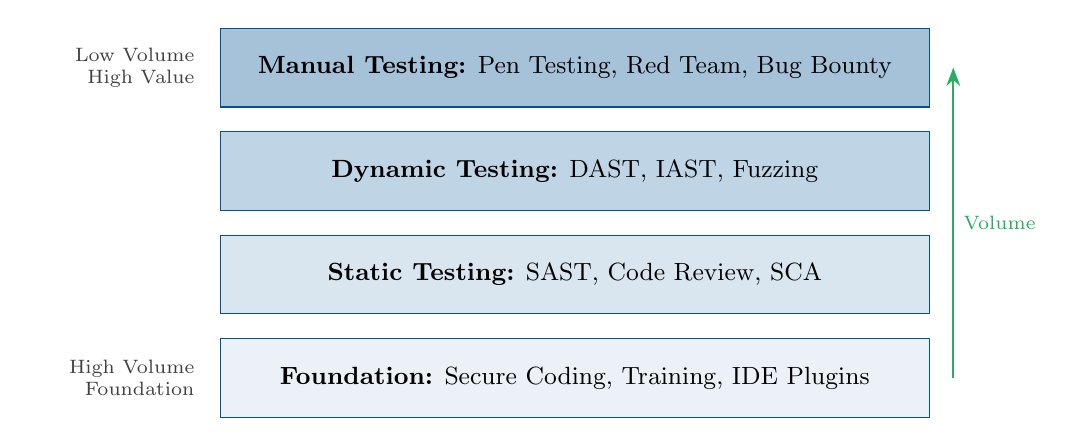
\begin{tikzpicture}[
    node distance=0.3cm,
    layer/.style={rectangle, draw=primaryblue, minimum width=9cm, minimum height=1cm, 
                  align=center, font=\small}
]
    % Layers
    \node[layer, fill=primaryblue!35] (manual) {\textbf{Manual Testing:} Pen Testing, Red Team, Bug Bounty};
    \node[layer, fill=primaryblue!25, below=of manual] (dynamic) {\textbf{Dynamic Testing:} DAST, IAST, Fuzzing};
    \node[layer, fill=primaryblue!15, below=of dynamic] (static) {\textbf{Static Testing:} SAST, Code Review, SCA};
    \node[layer, fill=primaryblue!8, below=of static] (foundation) {\textbf{Foundation:} Secure Coding, Training, IDE Plugins};
    
    % Annotations
    \node[left=0.2cm of manual, font=\scriptsize\color{darkgray}, text width=2cm, align=right] {Low Volume\\High Value};
    \node[left=0.2cm of foundation, font=\scriptsize\color{darkgray}, text width=2cm, align=right] {High Volume\\Foundation};
    
    % Arrow indicating volume
    \draw[-{Stealth}, thick, accentgreen] ([xshift=0.3cm]foundation.east) -- node[right, font=\scriptsize] {Volume} ([xshift=0.3cm]manual.east);
\end{tikzpicture}
\caption{Security Testing Coverage Pyramid}
\label{fig:testing-pyramid}
\end{figure}

\clearpage
\subsection{Automated Security Testing}

\subsubsection{CI/CD Integration}

Security testing must be integrated into continuous integration and continuous deployment pipelines to provide immediate feedback and enforce security gates.

\begin{table}[H]
\centering
\renewcommand{\arraystretch}{1.3}
\begin{tabularx}{\textwidth}{>{\bfseries}p{2.5cm} p{3.5cm} X}
\toprule
\textbf{Pipeline Stage} & \textbf{Security Tests} & \textbf{Gate Criteria} \\
\midrule
Pre-Commit & Secrets scanning, linting & Block commit if secrets detected \\
Build & SAST, SCA, container scanning & No critical findings; high findings reviewed \\
Test & DAST, IAST, security unit tests & No critical findings; test coverage met \\
Pre-Deploy & Configuration scanning, final SAST & All gates passed; approval obtained \\
Post-Deploy & Smoke tests, baseline validation & Security controls operational \\
\bottomrule
\end{tabularx}
\caption{CI/CD Security Integration Points}
\label{tab:cicd-security}
\end{table}

\subsubsection{Scan Scheduling and Triggers}

\begin{table}[H]
\centering
\renewcommand{\arraystretch}{1.3}
\begin{tabularx}{\textwidth}{>{\bfseries}p{2.5cm} p{4cm} X}
\toprule
\textbf{Test Type} & \textbf{Trigger} & \textbf{Additional Schedule} \\
\midrule
SAST & Every commit/pull request & Full repository scan weekly \\
SCA & Every build & Continuous monitoring for new CVEs \\
Secrets Scan & Pre-commit hook; every build & Weekly full repository scan \\
DAST & Deploy to test environment & Weekly production scan \\
Container Scan & Every image build & Daily scan of deployed images \\
Config Scan & Every deployment & Daily compliance check \\
\bottomrule
\end{tabularx}
\caption{Security Scan Scheduling}
\label{tab:scan-schedule}
\end{table}

\clearpage
\subsection{Manual Security Testing}

\subsubsection{Penetration Testing Methodology}

Penetration tests follow a structured methodology regardless of internal or external execution:

\begin{enumerate}[leftmargin=2em]
    \item \textbf{Scoping:} Define test boundaries, objectives, rules of engagement, and success criteria
    \item \textbf{Reconnaissance:} Gather information about target applications and infrastructure
    \item \textbf{Vulnerability Discovery:} Identify potential vulnerabilities through manual and automated techniques
    \item \textbf{Exploitation:} Attempt to exploit identified vulnerabilities to demonstrate impact
    \item \textbf{Post-Exploitation:} Assess potential for lateral movement and additional compromise
    \item \textbf{Reporting:} Document findings with severity ratings, evidence, and remediation guidance
    \item \textbf{Remediation Validation:} Verify that fixes effectively address identified vulnerabilities
\end{enumerate}

\subsubsection{Red Team Exercises}

Red team exercises simulate sophisticated adversary attacks against the organization's applications and infrastructure. Unlike penetration testing, red team exercises:

\begin{itemize}[leftmargin=2em]
    \item Focus on objectives rather than vulnerability enumeration
    \item Test detection and response capabilities alongside prevention
    \item Use stealth and evasion techniques
    \item May span extended timeframes
    \item Simulate realistic threat actor tactics, techniques, and procedures
\end{itemize}

Red team exercises are recommended annually for Tier 1 applications and critical infrastructure.

\clearpage
\subsubsection{Bug Bounty Program}

Bug bounty programs leverage external security researchers to identify vulnerabilities. Program structure:

\begin{keyconceptbox}[Bug Bounty Program Structure]
\textbf{Scope Definition:}

\begin{itemize}[leftmargin=1.5em, itemsep=0.1em]
    \item In-scope applications and domains
    \item Out-of-scope areas and prohibited activities
    \item Qualifying vulnerability types
    \item Testing guidelines and rules of engagement
\end{itemize}

\textbf{Reward Structure:}

\begin{itemize}[leftmargin=1.5em, itemsep=0.1em]
    \item Tiered rewards based on severity and impact
    \item Clear criteria for reward determination
    \item Bonus criteria for exceptional findings
    \item Timeline for reward payment
\end{itemize}

\textbf{Operational Process:}

\begin{itemize}[leftmargin=1.5em, itemsep=0.1em]
    \item Submission intake and triage process
    \item Response time commitments
    \item Communication protocols with researchers
    \item Disclosure coordination procedures
\end{itemize}
\end{keyconceptbox}

\subsection{Vulnerability Severity Classification}

All security findings are classified using a consistent severity framework:

\begin{table}[H]
\centering
\renewcommand{\arraystretch}{1.3}
\begin{tabularx}{\textwidth}{>{\bfseries\centering\arraybackslash}p{2.5cm} >{\centering\arraybackslash}p{2cm} X}
\toprule
\textbf{Severity} & \textbf{CVSS Range} & \textbf{Description and Examples} \\
\midrule
Critical & 9.0 -- 10.0 & Immediate, severe impact; trivial exploitation. Examples: unauthenticated RCE, SQL injection with full database access, authentication bypass to admin \\
High & 7.0 -- 8.9 & Significant impact; exploitation likely. Examples: stored XSS affecting multiple users, privilege escalation, significant data exposure \\
Medium & 4.0 -- 6.9 & Moderate impact; exploitation requires conditions. Examples: reflected XSS, CSRF, information disclosure of moderate sensitivity \\
Low & 0.1 -- 3.9 & Limited impact; difficult exploitation. Examples: verbose error messages, minor information disclosure, missing security headers \\
Info & N/A & Best practice recommendations; no direct security impact \\
\bottomrule
\end{tabularx}
\caption{Vulnerability Severity Classification}
\label{tab:severity-classification}
\end{table}

% ============================================================================
% SECTION 6: VULNERABILITY MANAGEMENT
% ============================================================================
\clearpage
\section{Vulnerability Management}

Vulnerability management encompasses the processes for identifying, assessing, prioritizing, remediating, and reporting security vulnerabilities across the application portfolio. Effective vulnerability management is essential for reducing organizational risk and demonstrating due diligence.

\subsection{Vulnerability Management Lifecycle}

\begin{figure}[H]
\centering
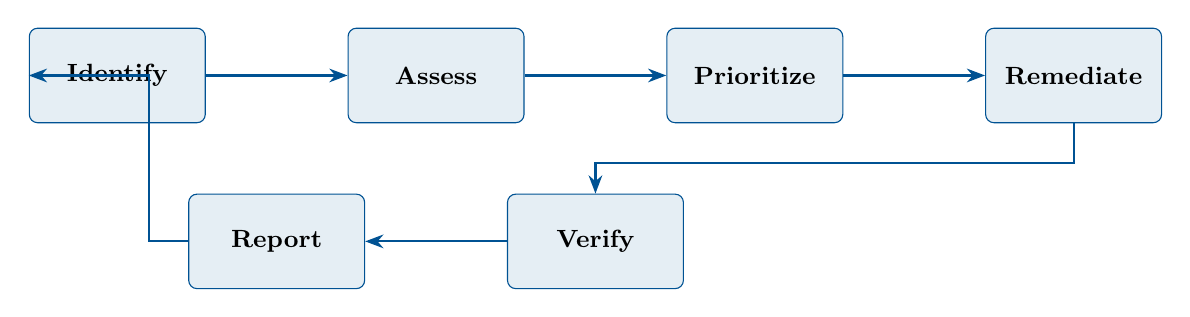
\begin{tikzpicture}[
    node distance=1.8cm,
    box/.style={rectangle, draw=primaryblue, fill=primaryblue!10, 
                text width=2cm, minimum height=1.2cm, align=center,
                rounded corners=3pt, font=\small\bfseries},
    arrow/.style={-{Stealth[scale=1]}, thick, primaryblue}
]
    \node[box] (identify) {Identify};
    \node[box, right=of identify] (assess) {Assess};
    \node[box, right=of assess] (prioritize) {Prioritize};
    \node[box, right=of prioritize] (remediate) {Remediate};
    \node[box, below=1.5cm of $(assess)!0.5!(prioritize)$] (verify) {Verify};
    \node[box, left=of verify] (report) {Report};
    
    \draw[arrow] (identify) -- (assess);
    \draw[arrow] (assess) -- (prioritize);
    \draw[arrow] (prioritize) -- (remediate);
    \draw[arrow] (remediate.south) -- ++(0,-0.5) -| (verify);
    \draw[arrow] (verify) -- (report);
    \draw[arrow] (report.west) -- ++(-0.5,0) |- (identify.west);
\end{tikzpicture}
\caption{Vulnerability Management Lifecycle}
\label{fig:vuln-lifecycle}
\end{figure}

\subsection{Vulnerability Identification}

Vulnerabilities are identified through multiple channels:

\begin{table}[H]
\centering
\renewcommand{\arraystretch}{1.3}
\begin{tabularx}{\textwidth}{>{\bfseries}p{3.5cm} X}
\toprule
\textbf{Source} & \textbf{Description} \\
\midrule
Automated Scanning & SAST, DAST, SCA, IAST, infrastructure scanning \\
Manual Testing & Penetration testing, code review, security assessments \\
External Research & Bug bounty submissions, responsible disclosure \\
Threat Intelligence & Vendor advisories, CVE publications, security bulletins \\
Internal Discovery & Developer reports, operations team findings, incident investigations \\
Third-Party Assessments & Customer security assessments, audit findings, compliance reviews \\
\bottomrule
\end{tabularx}
\caption{Vulnerability Identification Sources}
\label{tab:vuln-sources}
\end{table}

\clearpage
\subsection{Vulnerability Assessment and Prioritization}

Raw vulnerability data must be assessed and prioritized to focus remediation efforts on the highest-risk issues.

\subsubsection{Assessment Factors}

\begin{table}[H]
\centering
\renewcommand{\arraystretch}{1.3}
\begin{tabularx}{\textwidth}{>{\bfseries}p{3cm} X}
\toprule
\textbf{Factor} & \textbf{Considerations} \\
\midrule
Technical Severity & CVSS base score; attack complexity; required privileges \\
Exploitability & Exploit availability; active exploitation; ease of exploitation \\
Asset Criticality & Application tier; data sensitivity; business impact \\
Exposure & Internet-facing vs. internal; network accessibility; attack surface \\
Compensating Controls & Existing mitigations; defense in depth; monitoring coverage \\
Business Context & Regulatory implications; customer impact; reputational risk \\
\bottomrule
\end{tabularx}
\caption{Vulnerability Assessment Factors}
\label{tab:vuln-factors}
\end{table}

\subsubsection{Prioritization Model}

The organization uses a risk-based prioritization model that considers both technical severity and business context:

\[ \text{Priority Score} = \text{Technical Severity} \times \text{Asset Criticality} \times \text{Exposure Factor} \]

\begin{table}[H]
\centering
\renewcommand{\arraystretch}{1.3}
\begin{tabularx}{\textwidth}{>{\bfseries}p{2cm} >{\centering\arraybackslash}p{2.5cm} X}
\toprule
\textbf{Priority} & \textbf{Score Range} & \textbf{Treatment} \\
\midrule
P1 & 75 -- 100 & Immediate response; emergency remediation \\
P2 & 50 -- 74 & Urgent; next sprint/release \\
P3 & 25 -- 49 & Standard; scheduled remediation \\
P4 & 1 -- 24 & Low; address as capacity permits \\
\bottomrule
\end{tabularx}
\caption{Vulnerability Priority Levels}
\label{tab:vuln-priority}
\end{table}

\clearpage
\subsection{Remediation Requirements}

\subsubsection{Service Level Agreements}

Vulnerability remediation must occur within defined SLA timeframes based on priority:

\begin{alertbox}[Remediation SLA Requirements]
\begin{center}
\renewcommand{\arraystretch}{1.4}
\begin{tabular}{l c c}
\toprule
\textbf{Priority} & \textbf{Internet-Facing} & \textbf{Internal} \\
\midrule
P1 (Critical) & 24 -- 72 hours & 7 days \\
P2 (High) & 7 days & 14 days \\
P3 (Medium) & 30 days & 60 days \\
P4 (Low) & 90 days & 180 days \\
\bottomrule
\end{tabular}
\end{center}
\end{alertbox}

SLA timers begin when a vulnerability is confirmed and assigned. Extensions require documented approval according to the exception management process.

\subsubsection{Remediation Options}

Multiple approaches exist for addressing vulnerabilities:

\begin{enumerate}[leftmargin=2em]
    \item \textbf{Fix:} Correct the underlying vulnerability through code or configuration change (preferred)
    \item \textbf{Patch:} Apply vendor-supplied security patch
    \item \textbf{Upgrade:} Update to a version where the vulnerability is addressed
    \item \textbf{Mitigate:} Implement compensating controls that reduce risk without fixing root cause
    \item \textbf{Accept:} Document acceptance of residual risk (requires approval per exception process)
    \item \textbf{Retire:} Decommission the vulnerable component or application
\end{enumerate}

\subsection{Verification and Closure}

All remediated vulnerabilities require verification before closure:

\begin{itemize}[leftmargin=2em]
    \item Automated rescan confirming vulnerability no longer detected
    \item Manual verification for complex vulnerabilities
    \item Regression testing to ensure fix does not introduce new issues
    \item Documentation of remediation approach
    \item Update of tracking system with closure evidence
\end{itemize}

\clearpage
\subsection{Vulnerability Tracking and Reporting}

\subsubsection{Tracking Requirements}

All vulnerabilities are tracked in a centralized vulnerability management system with:

\begin{itemize}[leftmargin=2em]
    \item Unique identifier for each vulnerability
    \item Source, discovery date, and discoverer
    \item Affected application and component
    \item Technical details and evidence
    \item Severity and priority classification
    \item Assigned owner and remediation team
    \item SLA due date and current status
    \item Remediation history and closure evidence
\end{itemize}

\subsubsection{Reporting Cadence}

\begin{table}[H]
\centering
\renewcommand{\arraystretch}{1.3}
\begin{tabularx}{\textwidth}{>{\bfseries}p{3cm} p{3cm} X}
\toprule
\textbf{Report} & \textbf{Frequency} & \textbf{Audience} \\
\midrule
Operational Dashboard & Real-time & Application Security team \\
Development Team Report & Weekly & Development teams \\
Management Summary & Monthly & IT leadership \\
Executive Report & Quarterly & Steering Committee, Executives \\
Compliance Report & Per requirement & Auditors, Regulators \\
\bottomrule
\end{tabularx}
\caption{Vulnerability Reporting Cadence}
\label{tab:vuln-reporting}
\end{table}

% ============================================================================
% SECTION 7: THIRD-PARTY AND SUPPLY CHAIN SECURITY
% ============================================================================
\clearpage
\section{Third-Party and Supply Chain Security}

Modern applications extensively rely on third-party code, including commercial software, open-source libraries, cloud services, and external APIs. This section establishes requirements for managing security risks throughout the software supply chain.

\subsection{Supply Chain Risk Landscape}

\begin{figure}[H]
\centering
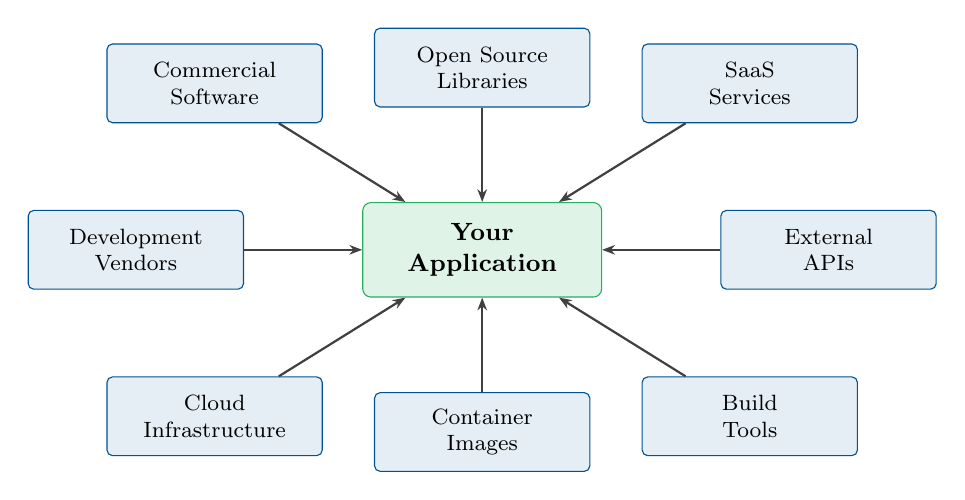
\begin{tikzpicture}[
    node distance=0.8cm,
    box/.style={rectangle, draw=primaryblue, fill=primaryblue!10, 
                text width=2.5cm, minimum height=1cm, align=center,
                rounded corners=2pt, font=\footnotesize},
    center/.style={rectangle, draw=accentgreen, fill=accentgreen!15, 
                text width=2.8cm, minimum height=1.2cm, align=center,
                rounded corners=3pt, font=\small\bfseries},
    arrow/.style={-{Stealth[scale=0.7]}, thick, darkgray}
]
    \node[center] (app) {Your\\Application};
    
    \node[box, above left=1cm and 0.5cm of app] (cots) {Commercial\\Software};
    \node[box, above=1.2cm of app] (oss) {Open Source\\Libraries};
    \node[box, above right=1cm and 0.5cm of app] (saas) {SaaS\\Services};
    \node[box, left=1.5cm of app] (vendor) {Development\\Vendors};
    \node[box, right=1.5cm of app] (api) {External\\APIs};
    \node[box, below left=1cm and 0.5cm of app] (cloud) {Cloud\\Infrastructure};
    \node[box, below=1.2cm of app] (container) {Container\\Images};
    \node[box, below right=1cm and 0.5cm of app] (tools) {Build\\Tools};
    
    \draw[arrow] (cots) -- (app);
    \draw[arrow] (oss) -- (app);
    \draw[arrow] (saas) -- (app);
    \draw[arrow] (vendor) -- (app);
    \draw[arrow] (api) -- (app);
    \draw[arrow] (cloud) -- (app);
    \draw[arrow] (container) -- (app);
    \draw[arrow] (tools) -- (app);
\end{tikzpicture}
\caption{Software Supply Chain Components}
\label{fig:supply-chain}
\end{figure}

\subsection{Vendor Security Assessment}

\subsubsection{Assessment Requirements}

Third-party vendors providing software, services, or access to organizational data must undergo security assessment proportionate to risk:

\begin{table}[H]
\centering
\renewcommand{\arraystretch}{1.3}
\begin{tabularx}{\textwidth}{>{\bfseries}p{2cm} p{4cm} X}
\toprule
\textbf{Risk Tier} & \textbf{Criteria} & \textbf{Assessment Requirements} \\
\midrule
Critical & Processes sensitive data; critical infrastructure; high access & Full security assessment; on-site review option; contractual requirements; annual reassessment \\
High & Moderate data access; business-important service; integration with internal systems & Security questionnaire; evidence review; contractual requirements; reassessment every 2 years \\
Medium & Limited data access; replaceable service; minimal integration & Abbreviated questionnaire; certification review; standard terms \\
Low & No data access; commodity service; no integration & Self-attestation; standard terms \\
\bottomrule
\end{tabularx}
\caption{Vendor Security Assessment Tiers}
\label{tab:vendor-tiers}
\end{table}

\subsubsection{Assessment Process}

\begin{enumerate}[leftmargin=2em]
    \item \textbf{Risk Classification:} Determine vendor risk tier based on data access, integration, and business criticality
    \item \textbf{Questionnaire:} Distribute appropriate security questionnaire
    \item \textbf{Evidence Review:} Examine provided certifications, audit reports, and policies
    \item \textbf{Gap Analysis:} Identify gaps between vendor capabilities and organizational requirements
    \item \textbf{Risk Decision:} Accept, require remediation, or reject based on assessment results
    \item \textbf{Contractual Controls:} Negotiate appropriate security terms and requirements
    \item \textbf{Ongoing Monitoring:} Track vendor security posture throughout relationship
\end{enumerate}

\clearpage
\subsection{Open Source Security}

\subsubsection{Open Source Governance}

Open source usage requires governance to manage security, license, and quality risks:

\begin{policybox}[Open Source Governance Requirements]
\textbf{Pre-Adoption Review:}

\begin{itemize}[leftmargin=1.5em, itemsep=0.1em]
    \item Security history and vulnerability record
    \item Maintenance activity and community health
    \item License compatibility with intended use
    \item Code quality indicators
    \item Available alternatives comparison
\end{itemize}

\textbf{Ongoing Management:}

\begin{itemize}[leftmargin=1.5em, itemsep=0.1em]
    \item Continuous vulnerability monitoring via SCA
    \item Version currency tracking
    \item License change monitoring
    \item Maintainer and ownership changes
    \item End-of-life and abandonment detection
\end{itemize}

\textbf{Approved/Prohibited Lists:}

\begin{itemize}[leftmargin=1.5em, itemsep=0.1em]
    \item Maintain list of pre-approved components
    \item Document prohibited components with rationale
    \item Establish review process for new component requests
\end{itemize}
\end{policybox}

\subsubsection{Dependency Management}

Effective dependency management minimizes supply chain attack surface:

\begin{itemize}[leftmargin=2em]
    \item Pin dependency versions in production configurations
    \item Use lock files to ensure reproducible builds
    \item Prefer well-maintained dependencies with active security response
    \item Minimize dependency depth where practical
    \item Regularly audit for unused dependencies
    \item Implement dependency confusion protections
    \item Verify package integrity through checksums or signatures
\end{itemize}

\clearpage
\subsection{Software Bill of Materials (SBOM)}

\subsubsection{SBOM Requirements}

All applications must maintain current Software Bills of Materials documenting their components:

\begin{table}[H]
\centering
\renewcommand{\arraystretch}{1.3}
\begin{tabularx}{\textwidth}{>{\bfseries}p{3.5cm} X}
\toprule
\textbf{SBOM Element} & \textbf{Requirements} \\
\midrule
Format & Standard format (SPDX, CycloneDX, or SWID) \\
Content & All direct and transitive dependencies; version information; supplier; license \\
Generation & Automated generation during build process \\
Currency & Updated with every release \\
Storage & Retained in accessible repository with versioning \\
Sharing & Available for customer requests and regulatory requirements \\
Analysis & Integrated with vulnerability monitoring for continuous risk assessment \\
\bottomrule
\end{tabularx}
\caption{SBOM Requirements}
\label{tab:sbom-requirements}
\end{table}

\subsection{Build Pipeline Security}

Securing the build pipeline prevents supply chain attacks that compromise the software delivery process:

\begin{itemize}[leftmargin=2em]
    \item Secure configuration of CI/CD systems
    \item Access controls and audit logging for pipeline modifications
    \item Signed commits and verified contributor identity
    \item Artifact signing and verification
    \item Isolated build environments
    \item Dependency verification during build
    \item Pipeline-as-code with version control
    \item Regular security review of build configurations
\end{itemize}

% ============================================================================
% SECTION 8: SECURITY TRAINING AND AWARENESS
% ============================================================================
\clearpage
\section{Security Training and Awareness}

Security training and awareness programs build the human capabilities necessary for effective application security. This section defines requirements for role-based training, developer education, and security awareness.

\subsection{Training Program Objectives}

\begin{enumerate}[leftmargin=2em, itemsep=0.3em]
    \item Ensure all personnel understand their security responsibilities
    \item Equip developers with skills to write secure code
    \item Build specialized expertise within the security team
    \item Create a security-conscious organizational culture
    \item Meet compliance requirements for security training
    \item Reduce human-factor security incidents
\end{enumerate}

\subsection{Role-Based Training Requirements}

\begin{longtable}{>{\bfseries}p{3cm} p{4cm} p{3cm} p{2.5cm}}
\toprule
\textbf{Role} & \textbf{Required Training} & \textbf{Frequency} & \textbf{Duration} \\
\midrule
\endfirsthead
\toprule
\textbf{Role} & \textbf{Required Training} & \textbf{Frequency} & \textbf{Duration} \\
\midrule
\endhead
\bottomrule
\endfoot
All Employees & Security Awareness Fundamentals & Annual & 1 hour \\
Developers & Secure Coding Foundations & Annual & 4 hours \\
Developers & Language/Framework-Specific Security & At adoption & 2-4 hours \\
Security Champions & Advanced Application Security & Annual & 16+ hours \\
Security Team & Specialized Technical Training & Ongoing & Per plan \\
Architects & Security Architecture Principles & Annual & 8 hours \\
QA Engineers & Security Testing Fundamentals & Annual & 4 hours \\
Operations & Secure Operations and Monitoring & Annual & 4 hours \\
Management & Security Leadership & Annual & 2 hours \\
Executives & Executive Security Briefing & Annual & 1 hour \\
\end{longtable}

\clearpage
\subsection{Developer Security Training}

\subsubsection{Secure Coding Curriculum}

Developer security training covers:

\begin{keyconceptbox}[Developer Security Training Curriculum]
\textbf{Foundations:}

\begin{itemize}[leftmargin=1.5em, itemsep=0.1em]
    \item Security mindset and threat landscape
    \item Common vulnerability types and root causes
    \item Secure development lifecycle overview
    \item Security requirements and acceptance criteria
\end{itemize}

\textbf{Defensive Coding:}

\begin{itemize}[leftmargin=1.5em, itemsep=0.1em]
    \item Input validation and output encoding
    \item Authentication and session management
    \item Access control implementation
    \item Cryptography fundamentals and proper usage
    \item Error handling and logging
    \item Secure configuration
\end{itemize}

\textbf{Technology-Specific:}

\begin{itemize}[leftmargin=1.5em, itemsep=0.1em]
    \item Language-specific security features and pitfalls
    \item Framework security controls
    \item API security
    \item Cloud-native security considerations
\end{itemize}

\textbf{Practical Skills:}

\begin{itemize}[leftmargin=1.5em, itemsep=0.1em]
    \item Using security testing tools
    \item Interpreting and triaging security findings
    \item Threat modeling participation
    \item Security code review
\end{itemize}
\end{keyconceptbox}

\subsubsection{Training Delivery Methods}

Multiple delivery methods accommodate different learning styles and schedules:

\begin{itemize}[leftmargin=2em]
    \item Online self-paced modules for foundational content
    \item Instructor-led sessions for complex topics and hands-on exercises
    \item Capture-the-flag (CTF) exercises for practical skill building
    \item Lunch-and-learn sessions for topical updates
    \item Embedded learning through IDE plugins and code review feedback
    \item Secure coding challenges and competitions
    \item Post-incident training based on real events
\end{itemize}

\subsection{Security Champion Program Training}

Security Champions receive enhanced training to serve as security liaisons within development teams:

\begin{table}[H]
\centering
\renewcommand{\arraystretch}{1.3}
\begin{tabularx}{\textwidth}{>{\bfseries\raggedright\arraybackslash}p{2.3cm} X >{\centering\arraybackslash}p{2cm}}
\toprule
\textbf{Track} & \textbf{Topics} & \textbf{Hours} \\
\midrule
Foundation & Advanced secure coding; threat modeling; security architecture principles & 8 \\
Tools & In-depth security tool training; finding interpretation; triage techniques & 8 \\
Process & Security requirements; risk assessment; exception handling; metrics & 4 \\
Leadership & Influencing without authority; security communication; team coaching & 4 \\
\bottomrule
\end{tabularx}
\caption{Security Champion Training Tracks}
\label{tab:champion-training}
\end{table}

\subsection{Training Effectiveness Measurement}

Training effectiveness is measured through:

\begin{itemize}[leftmargin=2em]
    \item Completion rates and compliance tracking
    \item Knowledge assessments and certification examinations
    \item Practical skill demonstrations
    \item Vulnerability trends in trained teams' code
    \item Security Champion activity metrics
    \item Post-training surveys and feedback
    \item Correlation between training and security metrics
\end{itemize}

% ============================================================================
% SECTION 9: INCIDENT RESPONSE
% ============================================================================
\clearpage
\section{Application Security Incident Response}

Application security incident response addresses security events affecting applications, including exploitation of vulnerabilities, data breaches through application vectors, and unauthorized access via application weaknesses.

\subsection{Incident Response Objectives}

\begin{enumerate}[leftmargin=2em, itemsep=0.3em]
    \item Minimize impact of application security incidents
    \item Restore secure application operations quickly
    \item Preserve evidence for investigation and potential legal proceedings
    \item Identify root causes and prevent recurrence
    \item Meet notification requirements for affected parties
    \item Capture lessons learned for program improvement
\end{enumerate}

\subsection{Incident Classification}

Application security incidents are classified by severity to determine response urgency and escalation:

\begin{table}[H]
\centering
\renewcommand{\arraystretch}{1.3}
\begin{tabularx}{\textwidth}{>{\bfseries\centering\arraybackslash}p{2cm} X p{4cm}}
\toprule
\textbf{Severity} & \textbf{Criteria} & \textbf{Response Requirement} \\
\midrule
Critical & Active exploitation; significant data breach; critical system compromise & Immediate response; executive notification; war room activation \\
High & Likely exploitation; limited breach; high-value system affected & Response within 4 hours; management notification \\
Medium & Potential exploitation; suspicious activity; moderate impact & Response within 24 hours; standard process \\
Low & Minor security event; no evidence of exploitation; limited impact & Response within 72 hours; normal workflow \\
\bottomrule
\end{tabularx}
\caption{Incident Severity Classification}
\label{tab:incident-severity}
\end{table}

\subsection{Incident Response Process}

\begin{figure}[H]
\centering
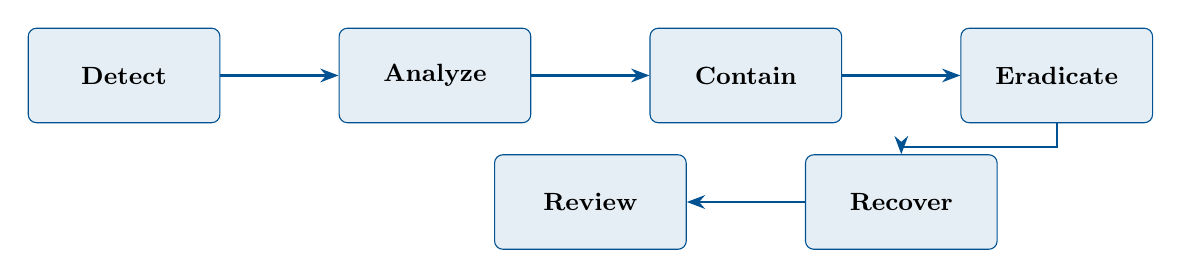
\begin{tikzpicture}[
    node distance=1.5cm,
    box/.style={rectangle, draw=primaryblue, fill=primaryblue!10, 
                text width=2.2cm, minimum height=1.2cm, align=center,
                rounded corners=3pt, font=\small\bfseries},
    arrow/.style={-{Stealth[scale=1]}, thick, primaryblue}
]
    \node[box] (detect) {Detect};
    \node[box, right=of detect] (analyze) {Analyze};
    \node[box, right=of analyze] (contain) {Contain};
    \node[box, right=of contain] (eradicate) {Eradicate};
    \node[box, below=1cm of $(contain)!0.5!(eradicate)$] (recover) {Recover};
    \node[box, left=of recover] (review) {Review};
    
    \draw[arrow] (detect) -- (analyze);
    \draw[arrow] (analyze) -- (contain);
    \draw[arrow] (contain) -- (eradicate);
    \draw[arrow] (eradicate.south) -- ++(0,-0.3) -| (recover);
    \draw[arrow] (recover) -- (review);
\end{tikzpicture}
\caption{Incident Response Phases}
\label{fig:ir-phases}
\end{figure}

\subsubsection{Detection}

Detection identifies potential application security incidents through:

\begin{itemize}[leftmargin=2em]
    \item Security monitoring and alerting systems
    \item Web application firewall events
    \item Runtime application protection alerts
    \item Anomaly detection systems
    \item User reports and help desk tickets
    \item External notifications (researchers, partners, customers)
    \item Penetration testing and security assessment discoveries
\end{itemize}

\subsubsection{Analysis}

Analysis determines incident scope, impact, and root cause:

\begin{itemize}[leftmargin=2em]
    \item Confirm whether a security incident has occurred
    \item Identify affected systems, data, and users
    \item Determine attack vector and exploitation method
    \item Assess data exposure and exfiltration
    \item Identify indicators of compromise
    \item Establish incident timeline
    \item Preserve evidence for investigation
\end{itemize}

\clearpage
\subsubsection{Containment}

Containment limits incident impact and prevents spread:

\begin{itemize}[leftmargin=2em]
    \item Isolate affected systems if necessary
    \item Block malicious traffic and attack sources
    \item Disable compromised accounts
    \item Implement emergency patches or configuration changes
    \item Activate additional monitoring
    \item Communicate with stakeholders
\end{itemize}

\subsubsection{Eradication}

Eradication removes the threat and addresses root cause:

\begin{itemize}[leftmargin=2em]
    \item Remove malicious code or backdoors
    \item Patch exploited vulnerabilities
    \item Reset compromised credentials
    \item Update security controls
    \item Verify complete removal of threat
\end{itemize}

\subsubsection{Recovery}

Recovery restores normal operations:

\begin{itemize}[leftmargin=2em]
    \item Restore systems from known-good state
    \item Verify system integrity before return to service
    \item Implement enhanced monitoring during recovery period
    \item Communicate recovery status to stakeholders
    \item Validate security controls functioning correctly
\end{itemize}

\subsubsection{Post-Incident Review}

Post-incident review captures lessons learned and improves future response:

\begin{itemize}[leftmargin=2em]
    \item Conduct formal post-incident review meeting
    \item Document incident timeline and response actions
    \item Identify what worked well and areas for improvement
    \item Determine root causes and contributing factors
    \item Define corrective actions with owners and deadlines
    \item Update incident response procedures as needed
    \item Share sanitized lessons learned across organization
\end{itemize}

\subsection{Communication Requirements}

\begin{table}[H]
\centering
\renewcommand{\arraystretch}{1.3}
\begin{tabularx}{\textwidth}{>{\bfseries\raggedright\arraybackslash}p{3.5cm} X}
\toprule
\textbf{Stakeholder} & \textbf{Communication Requirements} \\
\midrule
Exec.\ Leadership & Immediate notification for critical incidents; regular updates until resolved \\
Legal/Compliance & Notification when data breach suspected; guidance on regulatory requirements \\
Communications & Coordinate external messaging; prepare statements if needed \\
Affected Customers & Notification per regulatory requirements and contractual obligations \\
Regulators & Report within required timeframes based on jurisdiction and data type \\
Business Units & Keep informed of impact and recovery status \\
\bottomrule
\end{tabularx}
\caption{Incident Communication Requirements}
\label{tab:incident-comms}
\end{table}

% ============================================================================
% SECTION 10: COMPLIANCE AND AUDIT
% ============================================================================
\clearpage
\section{Compliance and Audit}

The Application Security Program supports organizational compliance with regulatory requirements, industry standards, and contractual obligations through documented controls, regular assessments, and audit-ready evidence.

\subsection{Compliance Framework}

\subsubsection{Regulatory Requirements}

The organization identifies and tracks applicable regulations affecting application security:

\begin{table}[H]
\centering
\renewcommand{\arraystretch}{1.3}
\begin{tabularx}{\textwidth}{>{\bfseries}p{3cm} X}
\toprule
\textbf{Regulation Type} & \textbf{Examples and Considerations} \\
\midrule
Data Protection & General data protection regulations; privacy laws; cross-border transfer requirements \\
Financial Services & Payment card security; financial reporting controls; trading system requirements \\
Healthcare & Protected health information; medical device security; healthcare interoperability \\
Government & Federal information security; defense contractor requirements; critical infrastructure protection \\
Industry-Specific & Telecommunications; energy sector; transportation security \\
\bottomrule
\end{tabularx}
\caption{Regulatory Requirement Categories}
\label{tab:regulatory-categories}
\end{table}

\subsubsection{Industry Standards}

The program aligns with recognized industry standards and frameworks:

\begin{itemize}[leftmargin=2em]
    \item OWASP Application Security Verification Standard (ASVS)
    \item NIST Secure Software Development Framework (SSDF)
    \item ISO/IEC 27034 Application Security
    \item Payment Card Industry Data Security Standard (PCI DSS)
    \item SOC 2 Trust Services Criteria
    \item Cloud Security Alliance controls
\end{itemize}

\clearpage
\subsection{Control Documentation}

\subsubsection{Control Library}

The Application Security Program maintains a control library documenting:

\begin{itemize}[leftmargin=2em]
    \item Control identifier and name
    \item Control objective and description
    \item Implementation guidance
    \item Testing procedures
    \item Evidence requirements
    \item Control owner
    \item Mapping to compliance requirements
    \item Related policies and procedures
\end{itemize}

\subsubsection{Evidence Management}

Compliance evidence must be systematically collected, retained, and accessible:

\begin{policybox}[Evidence Management Requirements]
\textbf{Evidence Types:}

\begin{itemize}[leftmargin=1.5em, itemsep=0.1em]
    \item Security scan reports (SAST, DAST, SCA)
    \item Penetration test reports
    \item Training completion records
    \item Policy acknowledgments
    \item Risk assessment documentation
    \item Exception records and approvals
    \item Incident response records
    \item Change management records
\end{itemize}

\textbf{Retention Requirements:}

\begin{itemize}[leftmargin=1.5em, itemsep=0.1em]
    \item Retain evidence for compliance period plus buffer (typically 3-7 years)
    \item Ensure evidence integrity and authenticity
    \item Maintain evidence accessibility for audit requests
    \item Protect evidence confidentiality appropriately
\end{itemize}
\end{policybox}

\clearpage
\subsection{Audit Support}

\subsubsection{Internal Audit}

Internal audit periodically assesses Application Security Program effectiveness:

\begin{itemize}[leftmargin=2em]
    \item Annual program audit covering governance, processes, and controls
    \item Targeted audits of specific program areas
    \item Follow-up on previous audit findings
    \item Coordination with enterprise internal audit function
\end{itemize}

\subsubsection{External Audit}

External audits from regulators, customers, and certification bodies require coordinated support:

\begin{itemize}[leftmargin=2em]
    \item Designated audit liaison within Application Security team
    \item Pre-audit preparation and evidence compilation
    \item Timely response to auditor requests
    \item Tracking and remediation of audit findings
    \item Management response documentation
\end{itemize}

\subsection{Compliance Monitoring}

Continuous compliance monitoring identifies deviations before they become audit findings:

\begin{itemize}[leftmargin=2em]
    \item Automated control testing where possible
    \item Regular self-assessments against control requirements
    \item Compliance dashboards tracking key indicators
    \item Trend analysis identifying degrading compliance
    \item Integration with vulnerability and configuration management
\end{itemize}

% ============================================================================
% SECTION 11: METRICS AND REPORTING
% ============================================================================
\clearpage
\section{Metrics and Reporting}

Metrics and reporting enable data-driven management of the Application Security Program by measuring performance, identifying trends, and communicating status to stakeholders.

\subsection{Metrics Framework}

\subsubsection{Metrics Categories}

\begin{table}[H]
\centering
\renewcommand{\arraystretch}{1.3}
\begin{tabularx}{\textwidth}{>{\bfseries}p{2.5cm} p{4cm} X}
\toprule
\textbf{Category} & \textbf{Purpose} & \textbf{Example Metrics} \\
\midrule
Coverage & Measure program reach and adoption & Percentage of applications with SAST; threat model coverage; training completion rate \\
Effectiveness & Assess control and process quality & Vulnerability escape rate; mean time to remediate; finding recurrence rate \\
Efficiency & Evaluate resource utilization & Security review cycle time; cost per vulnerability found; automation rate \\
Risk & Quantify security posture & Open critical vulnerabilities; risk score trends; exploited vulnerability count \\
Compliance & Track regulatory adherence & Compliance percentage; audit finding count; exception volume \\
\bottomrule
\end{tabularx}
\caption{Security Metrics Categories}
\label{tab:metrics-categories}
\end{table}

\clearpage
\subsection{Key Performance Indicators}

\subsubsection{Primary KPIs}

\begin{longtable}{>{\bfseries}p{4cm} p{5cm} p{4cm}}
\toprule
\textbf{Metric} & \textbf{Definition} & \textbf{Target} \\
\midrule
\endfirsthead
\toprule
\textbf{Metric} & \textbf{Definition} & \textbf{Target} \\
\midrule
\endhead
\bottomrule
\endfoot
SAST Coverage & Percentage of repositories with SAST integration & 100\% for Tier 1-2; 90\% overall \\
DAST Coverage & Percentage of web applications with DAST scanning & 100\% for Tier 1-2 \\
SCA Coverage & Percentage of applications with dependency scanning & 100\% \\
Critical Vuln MTTR & Mean time to remediate critical vulnerabilities & $<$ 72 hours \\
High Vuln MTTR & Mean time to remediate high vulnerabilities & $<$ 14 days \\
Vulnerability SLA Compliance & Percentage of vulnerabilities remediated within SLA & $>$ 95\% \\
Security Training Completion & Percentage of required training completed on time & $>$ 95\% \\
Threat Model Coverage & Percentage of Tier 1-2 applications with current threat models & 100\% \\
Security Gate Pass Rate & Percentage of releases passing security gates on first attempt & $>$ 80\% \\
Finding Recurrence Rate & Percentage of vulnerabilities that recur after remediation & $<$ 5\% \\
\end{longtable}

\subsubsection{Key Risk Indicators}

\begin{table}[H]
\centering
\renewcommand{\arraystretch}{1.3}
\begin{tabularx}{\textwidth}{>{\bfseries}p{4cm} X >{\centering\arraybackslash}p{2.5cm}}
\toprule
\textbf{Indicator} & \textbf{Risk Signal} & \textbf{Threshold} \\
\midrule
Aging Critical Vulnerabilities & Critical vulnerabilities open beyond SLA & $>$ 0 \\
Vulnerability Backlog Growth & Month-over-month increase in open vulnerabilities & $>$ 10\% \\
Security Exception Volume & Active security exceptions & $>$ 20 \\
Failed Security Gates & Releases blocked by security findings & $>$ 25\% \\
Unscanned Applications & Applications without recent security scanning & $>$ 5\% \\
Overdue Penetration Tests & Applications past due for penetration testing & $>$ 0 \\
\bottomrule
\end{tabularx}
\caption{Key Risk Indicators}
\label{tab:kris}
\end{table}

\subsection{Reporting Structure}

\subsubsection{Operational Reporting}

Operational reports support day-to-day program management:

\begin{itemize}[leftmargin=2em]
    \item Real-time dashboards showing current vulnerability status
    \item Daily scan result summaries
    \item SLA tracking and approaching deadline alerts
    \item Tool health and coverage reports
    \item Development team security scorecards
\end{itemize}

\subsubsection{Management Reporting}

Management reports provide oversight visibility:

\begin{itemize}[leftmargin=2em]
    \item Monthly program status reports
    \item Trend analysis and quarter-over-quarter comparisons
    \item Resource utilization and capacity reports
    \item Project status for security initiatives
    \item Risk register updates
\end{itemize}

\subsubsection{Executive Reporting}

Executive reports communicate strategic status:

\begin{itemize}[leftmargin=2em]
    \item Quarterly security posture summaries
    \item Key risk indicators and trends
    \item Significant incidents and responses
    \item Program maturity progress
    \item Budget and resource needs
    \item Strategic initiative status
\end{itemize}

\clearpage
\subsection{Continuous Improvement}

Metrics drive continuous improvement through:

\begin{enumerate}[leftmargin=2em]
    \item Regular review of metric trends to identify improvement opportunities
    \item Root cause analysis of negative trends
    \item Action planning and tracking for improvements
    \item Benchmark comparison against industry data
    \item Program retrospectives and lessons learned
    \item Feedback collection from stakeholders
    \item Annual program assessment and roadmap updates
\end{enumerate}

% ============================================================================
% SECTION 12: PROGRAM MATURITY
% ============================================================================
\clearpage
\section{Program Maturity}

Program maturity assessment provides a framework for understanding current capabilities, setting improvement priorities, and tracking progress over time.

\subsection{Maturity Model}

The Application Security Program maturity model defines five levels of capability:

\begin{figure}[H]
\centering
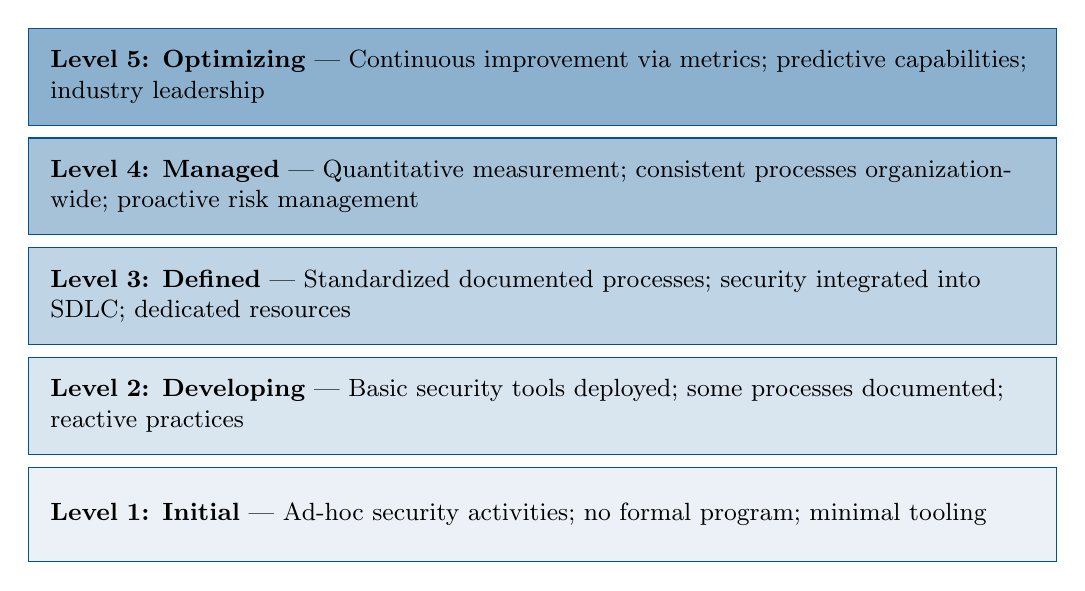
\begin{tikzpicture}[
    node distance=0.15cm,
    level/.style={rectangle, draw=primaryblue, minimum width=13cm, text width=12.5cm, minimum height=1.2cm, 
                  align=left, font=\small, inner sep=8pt}
]
    \node[level, fill=primaryblue!45] (l5) {\textbf{Level 5: Optimizing} --- Continuous improvement via metrics; predictive capabilities; industry leadership};
    \node[level, fill=primaryblue!35, below=of l5] (l4) {\textbf{Level 4: Managed} --- Quantitative measurement; consistent processes organization-wide; proactive risk management};
    \node[level, fill=primaryblue!25, below=of l4] (l3) {\textbf{Level 3: Defined} --- Standardized documented processes; security integrated into SDLC; dedicated resources};
    \node[level, fill=primaryblue!15, below=of l3] (l2) {\textbf{Level 2: Developing} --- Basic security tools deployed; some processes documented; reactive practices};
    \node[level, fill=primaryblue!8, below=of l2] (l1) {\textbf{Level 1: Initial} --- Ad-hoc security activities; no formal program; minimal tooling};
\end{tikzpicture}
\caption{Application Security Program Maturity Levels}
\label{fig:maturity-model}
\end{figure}

\clearpage
\subsection{Maturity Domains}

Maturity is assessed across multiple domains:

\begin{table}[H]
\centering
\renewcommand{\arraystretch}{1.3}
\begin{tabularx}{\textwidth}{>{\bfseries\raggedright\arraybackslash}p{4cm} X}
\toprule
\textbf{Domain} & \textbf{Assessment Areas} \\
\midrule
Governance & Strategy; policy; organizational structure; accountability; risk management \\
Secure Development & Requirements; design; coding practices; code review; developer tooling \\
Security Testing & SAST; DAST; SCA; penetration testing; test coverage; automation \\
Vulnerability Mgmt & Identification; prioritization; remediation; verification; tracking \\
Third-Party Security & Vendor assessment; open source governance; supply chain security; SBOM \\
Training & Role-based training; developer education; security champions; awareness \\
Incident Response & Detection; analysis; response; recovery; post-incident improvement \\
Metrics \& Reporting & Data collection; analysis; reporting; decision support \\
\bottomrule
\end{tabularx}
\caption{Maturity Assessment Domains}
\label{tab:maturity-domains}
\end{table}

\subsection{Maturity Assessment Process}

\begin{enumerate}[leftmargin=2em]
    \item \textbf{Self-Assessment:} Program team evaluates current state against maturity criteria
    \item \textbf{Evidence Review:} Validate self-assessment against documented evidence
    \item \textbf{Stakeholder Input:} Gather perspectives from development teams, operations, and management
    \item \textbf{Gap Analysis:} Identify gaps between current and target maturity levels
    \item \textbf{Roadmap Development:} Define initiatives to address gaps with priorities and timelines
    \item \textbf{Progress Tracking:} Monitor implementation and reassess periodically
\end{enumerate}

\clearpage
\subsection{Maturity Improvement Roadmap}

\begin{examplebox}[Sample Maturity Improvement Roadmap]
\textbf{Year 1: Foundation (Target: Level 2$\rightarrow$3)}

\begin{itemize}[leftmargin=1.5em, itemsep=0.1em]
    \item Establish formal governance structure and policies
    \item Deploy SAST and SCA across priority applications
    \item Implement vulnerability management process
    \item Launch developer security training program
    \item Define and begin tracking core metrics
\end{itemize}

\textbf{Year 2: Standardization (Target: Level 3)}

\begin{itemize}[leftmargin=1.5em, itemsep=0.1em]
    \item Achieve full SAST/SCA coverage for Tier 1-2 applications
    \item Integrate security testing into CI/CD pipelines
    \item Establish Security Champion program
    \item Implement threat modeling for critical applications
    \item Automate compliance evidence collection
\end{itemize}

\textbf{Year 3: Optimization (Target: Level 3$\rightarrow$4)}

\begin{itemize}[leftmargin=1.5em, itemsep=0.1em]
    \item Expand coverage to all applications
    \item Implement advanced testing (IAST, RASP)
    \item Mature metrics and reporting capabilities
    \item Establish continuous improvement processes
    \item Achieve consistent process execution organization-wide
\end{itemize}
\end{examplebox}

% ============================================================================
% SECTION 13: CONCLUSION
% ============================================================================
\clearpage
\section{Conclusion}

This Application Security Program provides the comprehensive framework necessary to systematically reduce application security risk across the enterprise. Success requires sustained commitment from executive leadership, adequate resource allocation, and cultural change that positions security as a shared responsibility rather than an obstacle to delivery.

\begin{summarybox}
\textbf{Program Success Factors:}

\textbf{1. Executive Commitment:} Visible leadership support, adequate resource allocation, and organizational authority for security requirements.

\textbf{2. Integration Over Addition:} Security activities embedded into existing workflows rather than bolted on as separate gates.

\textbf{3. Risk-Based Approach:} Focus resources on highest-risk applications and vulnerabilities rather than attempting uniform coverage.

\textbf{4. Developer Experience:} Security tools and processes that support rather than obstruct development productivity.

\textbf{5. Measurable Progress:} Clear metrics that demonstrate value and identify improvement opportunities.

\textbf{6. Continuous Improvement:} Regular assessment and evolution of program capabilities in response to changing threats and organizational needs.

\textbf{7. Cultural Change:} Building security awareness and capability throughout the organization, not just within a dedicated security team.
\end{summarybox}

Implementation of this program should be phased based on organizational readiness and priorities. Starting with governance foundations, critical application coverage, and developer enablement provides the base for progressive maturity improvement.

\vspace{1cm}

\begin{center}
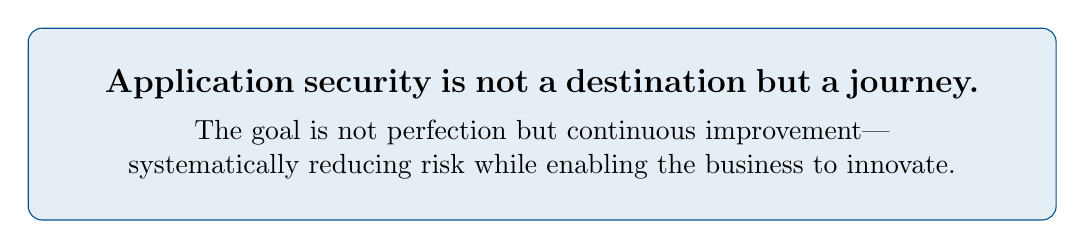
\begin{tikzpicture}
    \node[draw=primaryblue, fill=primaryblue!10, rounded corners=5pt, 
          text width=12cm, align=center, inner sep=15pt] {
        \textbf{\large Application security is not a destination but a journey.}\\[0.5em]
        {\normalsize The goal is not perfection but continuous improvement---\\systematically reducing risk while enabling the business to innovate.}
    };
\end{tikzpicture}
\end{center}

% ============================================================================
% APPENDICES
% ============================================================================
\newpage
\appendix

\clearpage
\section{Appendix A: Security Requirements Checklist}

\begin{longtable}{>{\bfseries\raggedright\arraybackslash}p{4cm} p{9cm}}
\toprule
\textbf{Category} & \textbf{Requirements} \\
\midrule
\endfirsthead
\toprule
\textbf{Category} & \textbf{Requirements} \\
\midrule
\endhead
\bottomrule
\endfoot
Authentication & Multi-factor authentication for sensitive functions; secure credential storage; account lockout after failed attempts; secure password reset; session timeout enforcement \\
Authorization & Role-based access control; least privilege implementation; authorization checks on all requests; segregation of duties for critical functions \\
Input Validation & Server-side validation for all input; whitelist validation where possible; parameterized database queries; proper encoding of output \\
Cryptography & Encryption of sensitive data at rest and in transit; approved algorithms only; proper key management; certificate validation \\
Error Handling & Secure error messages without sensitive information; comprehensive exception handling; appropriate logging of errors \\
Logging & Security event logging; log integrity protection; sufficient detail for investigation; log retention per policy \\
Session Mgmt & Secure session token generation; session binding to client; timeout enforcement; secure session termination \\
Data Protection & Data classification applied; encryption per classification; data minimization; secure deletion \\
Communication & TLS 1.2+ for all external communication; certificate validation; secure protocol configuration \\
Configuration & Secure defaults; hardening applied; removal of unnecessary features; change management \\
\end{longtable}

\clearpage
\section{Appendix B: Threat Modeling Template}

\begin{table}[H]
\centering
\renewcommand{\arraystretch}{1.3}
\begin{tabularx}{\textwidth}{>{\bfseries\raggedright\arraybackslash}p{4cm} X}
\toprule
\textbf{Section} & \textbf{Content} \\
\midrule
Application Overview & Name, purpose, owner, risk tier, technology stack \\
Architecture Desc. & Components, data flows, external dependencies, trust boundaries \\
Assets & Sensitive data, critical functions, valuable resources \\
Entry Points & External interfaces, APIs, user inputs, file uploads \\
Threat Actors & Relevant threat actors and their capabilities/motivations \\
Threats Identified & Threat ID, description, STRIDE category, affected assets \\
Vulnerabilities & Potential weaknesses that could enable threats \\
Countermeasures & Existing and proposed controls for each threat \\
Risk Assessment & Likelihood, impact, and priority for each threat \\
Residual Risk & Remaining risk after countermeasures \\
Action Items & Required actions, owners, and target dates \\
\bottomrule
\end{tabularx}
\caption{Threat Model Document Template}
\label{tab:threat-model-template}
\end{table}

\clearpage
\section{Appendix C: Vulnerability Report Template}

\begin{table}[H]
\centering
\renewcommand{\arraystretch}{1.3}
\begin{tabularx}{\textwidth}{>{\bfseries\raggedright\arraybackslash}p{4cm} X}
\toprule
\textbf{Field} & \textbf{Description} \\
\midrule
Vulnerability ID & Unique identifier \\
Title & Brief descriptive title \\
Discovery Date & Date vulnerability was identified \\
Source & How the vulnerability was discovered \\
Affected Application & Application name and version \\
Affected Component & Specific module, file, or function \\
Vulnerability Type & Classification (e.g., SQL injection, XSS) \\
Description & Detailed technical description \\
Proof of Concept & Steps to reproduce; evidence \\
Impact Assessment & Potential business and technical impact \\
CVSS Score & Common Vulnerability Scoring System rating \\
Severity & Critical/High/Medium/Low classification \\
Priority & Remediation priority assignment \\
Remediation Guidance & Recommended fix approach \\
Assigned Owner & Person responsible for remediation \\
SLA Due Date & Remediation deadline \\
Status & Current status in remediation workflow \\
Resolution & How the vulnerability was addressed \\
Verification & Evidence that fix is effective \\
\bottomrule
\end{tabularx}
\caption{Vulnerability Report Template}
\label{tab:vuln-template}
\end{table}

\clearpage
\section{Appendix D: Security Tool Categories}

\begin{longtable}{>{\bfseries}p{1cm} >{\raggedright\arraybackslash}p{3.2cm} >{\raggedright\arraybackslash}p{8.1cm}}
\toprule
\textbf{Acro.} & \textbf{Full Name} & \textbf{Description} \\
\midrule
\endfirsthead
\toprule
\textbf{Acro.} & \textbf{Full Name} & \textbf{Description} \\
\midrule
\endhead
\bottomrule
\endfoot
SAST & Static App Sec Testing & Analyzes source code or binaries for vulnerabilities without execution \\
DAST & Dynamic App Sec Testing & Tests running applications by simulating attacks \\
IAST & Interactive App Sec Testing & Combines static and dynamic analysis using runtime agents \\
SCA & Software Composition Analysis & Identifies vulnerabilities in third-party components \\
RASP & Runtime App Self-Protection & Provides runtime protection from within the application \\
WAF & Web App Firewall & Filters and monitors HTTP traffic to protect web applications \\
ASPM & App Security Posture Mgmt & Unified visibility and risk management across app security \\
SBOM & Software Bill of Materials & Inventory of all software components \\
AST & App Security Testing & General category encompassing SAST, DAST, IAST \\
CSPM & Cloud Security Posture Mgmt & Monitors cloud configurations for security issues \\
\end{longtable}

\clearpage
\section{Appendix E: Reference Standards and Frameworks}

\begin{itemize}[leftmargin=2em, itemsep=0.4em]
    \item \textbf{OWASP ASVS} --- Application Security Verification Standard
    \item \textbf{OWASP SAMM} --- Software Assurance Maturity Model
    \item \textbf{NIST SSDF} --- Secure Software Development Framework (SP 800-218)
    \item \textbf{NIST CSF} --- Cybersecurity Framework
    \item \textbf{ISO/IEC 27034} --- Application Security
    \item \textbf{BSIMM} --- Building Security In Maturity Model
    \item \textbf{CIS Controls} --- Center for Internet Security Controls
    \item \textbf{MITRE ATT\&CK} --- Adversarial Tactics, Techniques, and Common Knowledge
    \item \textbf{STRIDE} --- Spoofing, Tampering, Repudiation, Information Disclosure, Denial of Service, Elevation of Privilege
    \item \textbf{CVSS} --- Common Vulnerability Scoring System
\end{itemize}

\end{document}